\documentclass[a4paper, 11pt, oneside, polutonikogreek, english]{article}
\usepackage[utf8]{inputenc}
\usepackage[T1]{fontenc}
\usepackage{gfsneohellenic}
% Load encoding definitions (after font package)
\usepackage[dvipsnames]{xcolor}
\usepackage{eso-pic,graphicx}
\usepackage[top=82mm, bottom=82mm, outer=50mm, inner=50mm]{geometry}
\setlength{\columnsep}{90pt}
\usepackage{textalpha}
\usepackage{bbding}
\usepackage{listings}
\lstset{basicstyle=\ttfamily}
\usepackage{bbding}
\usepackage{listings}
% Babel package:
\usepackage[greek]{babel}
% With XeTeX$\$LuaTeX, load fontspec after babel to use Unicode
% fonts for Latin script and LGR for Greek:
\ifdefined\luatexversion \usepackage{fontspec}\fi
\ifdefined\XeTeXrevision \usepackage{fontspec}\fi

% ```Lipsiakos"' italic font `cbleipzig`:
\newcommand*{\lishape}{\fontencoding{LGR}\fontfamily{cmr}%
		 \fontshape{li}\selectfont}
\DeclareTextFontCommand{\textli}{\lishape}
\usepackage{booktabs}
\usepackage{fancyhdr}
\usepackage{graphicx}
\graphicspath{ {./ } }
\usepackage[figurename=]{caption}
\usepackage{float}
\usepackage{microtype}
\setlength{\emergencystretch}{15pt}
\usepackage{sectsty}
\usepackage[titles]{tocloft}

\sectionfont{\Large}
\subsectionfont{\large}

\usepackage{setspace}
\onehalfspacing
% change color of text, example replace all \color{Goldenrod} with \color{lightgray}

\makeatletter % change only the display of \thepage, but not \thepage itself:
\patchcmd{\ps@plain}{\thepage}{\bfseries\large\color{Black}{\thepage}}{}{}
\makeatother

\color{Black}

\begin{document}
\renewcommand{\thefigure}{{\bfseries\arabic{figure}}}
\renewcommand\thefootnote{\tiny{\arabic{footnote}}}
\let\oldfootnote\footnote
    \renewcommand{\footnote}[1]{\oldfootnote{\bfseries\footnotesize#1}}
    
\bfseries
\pagestyle{plain} % after changing a pagestyle command, it's necessary to invoke it explicitly
\AddToShipoutPictureBG{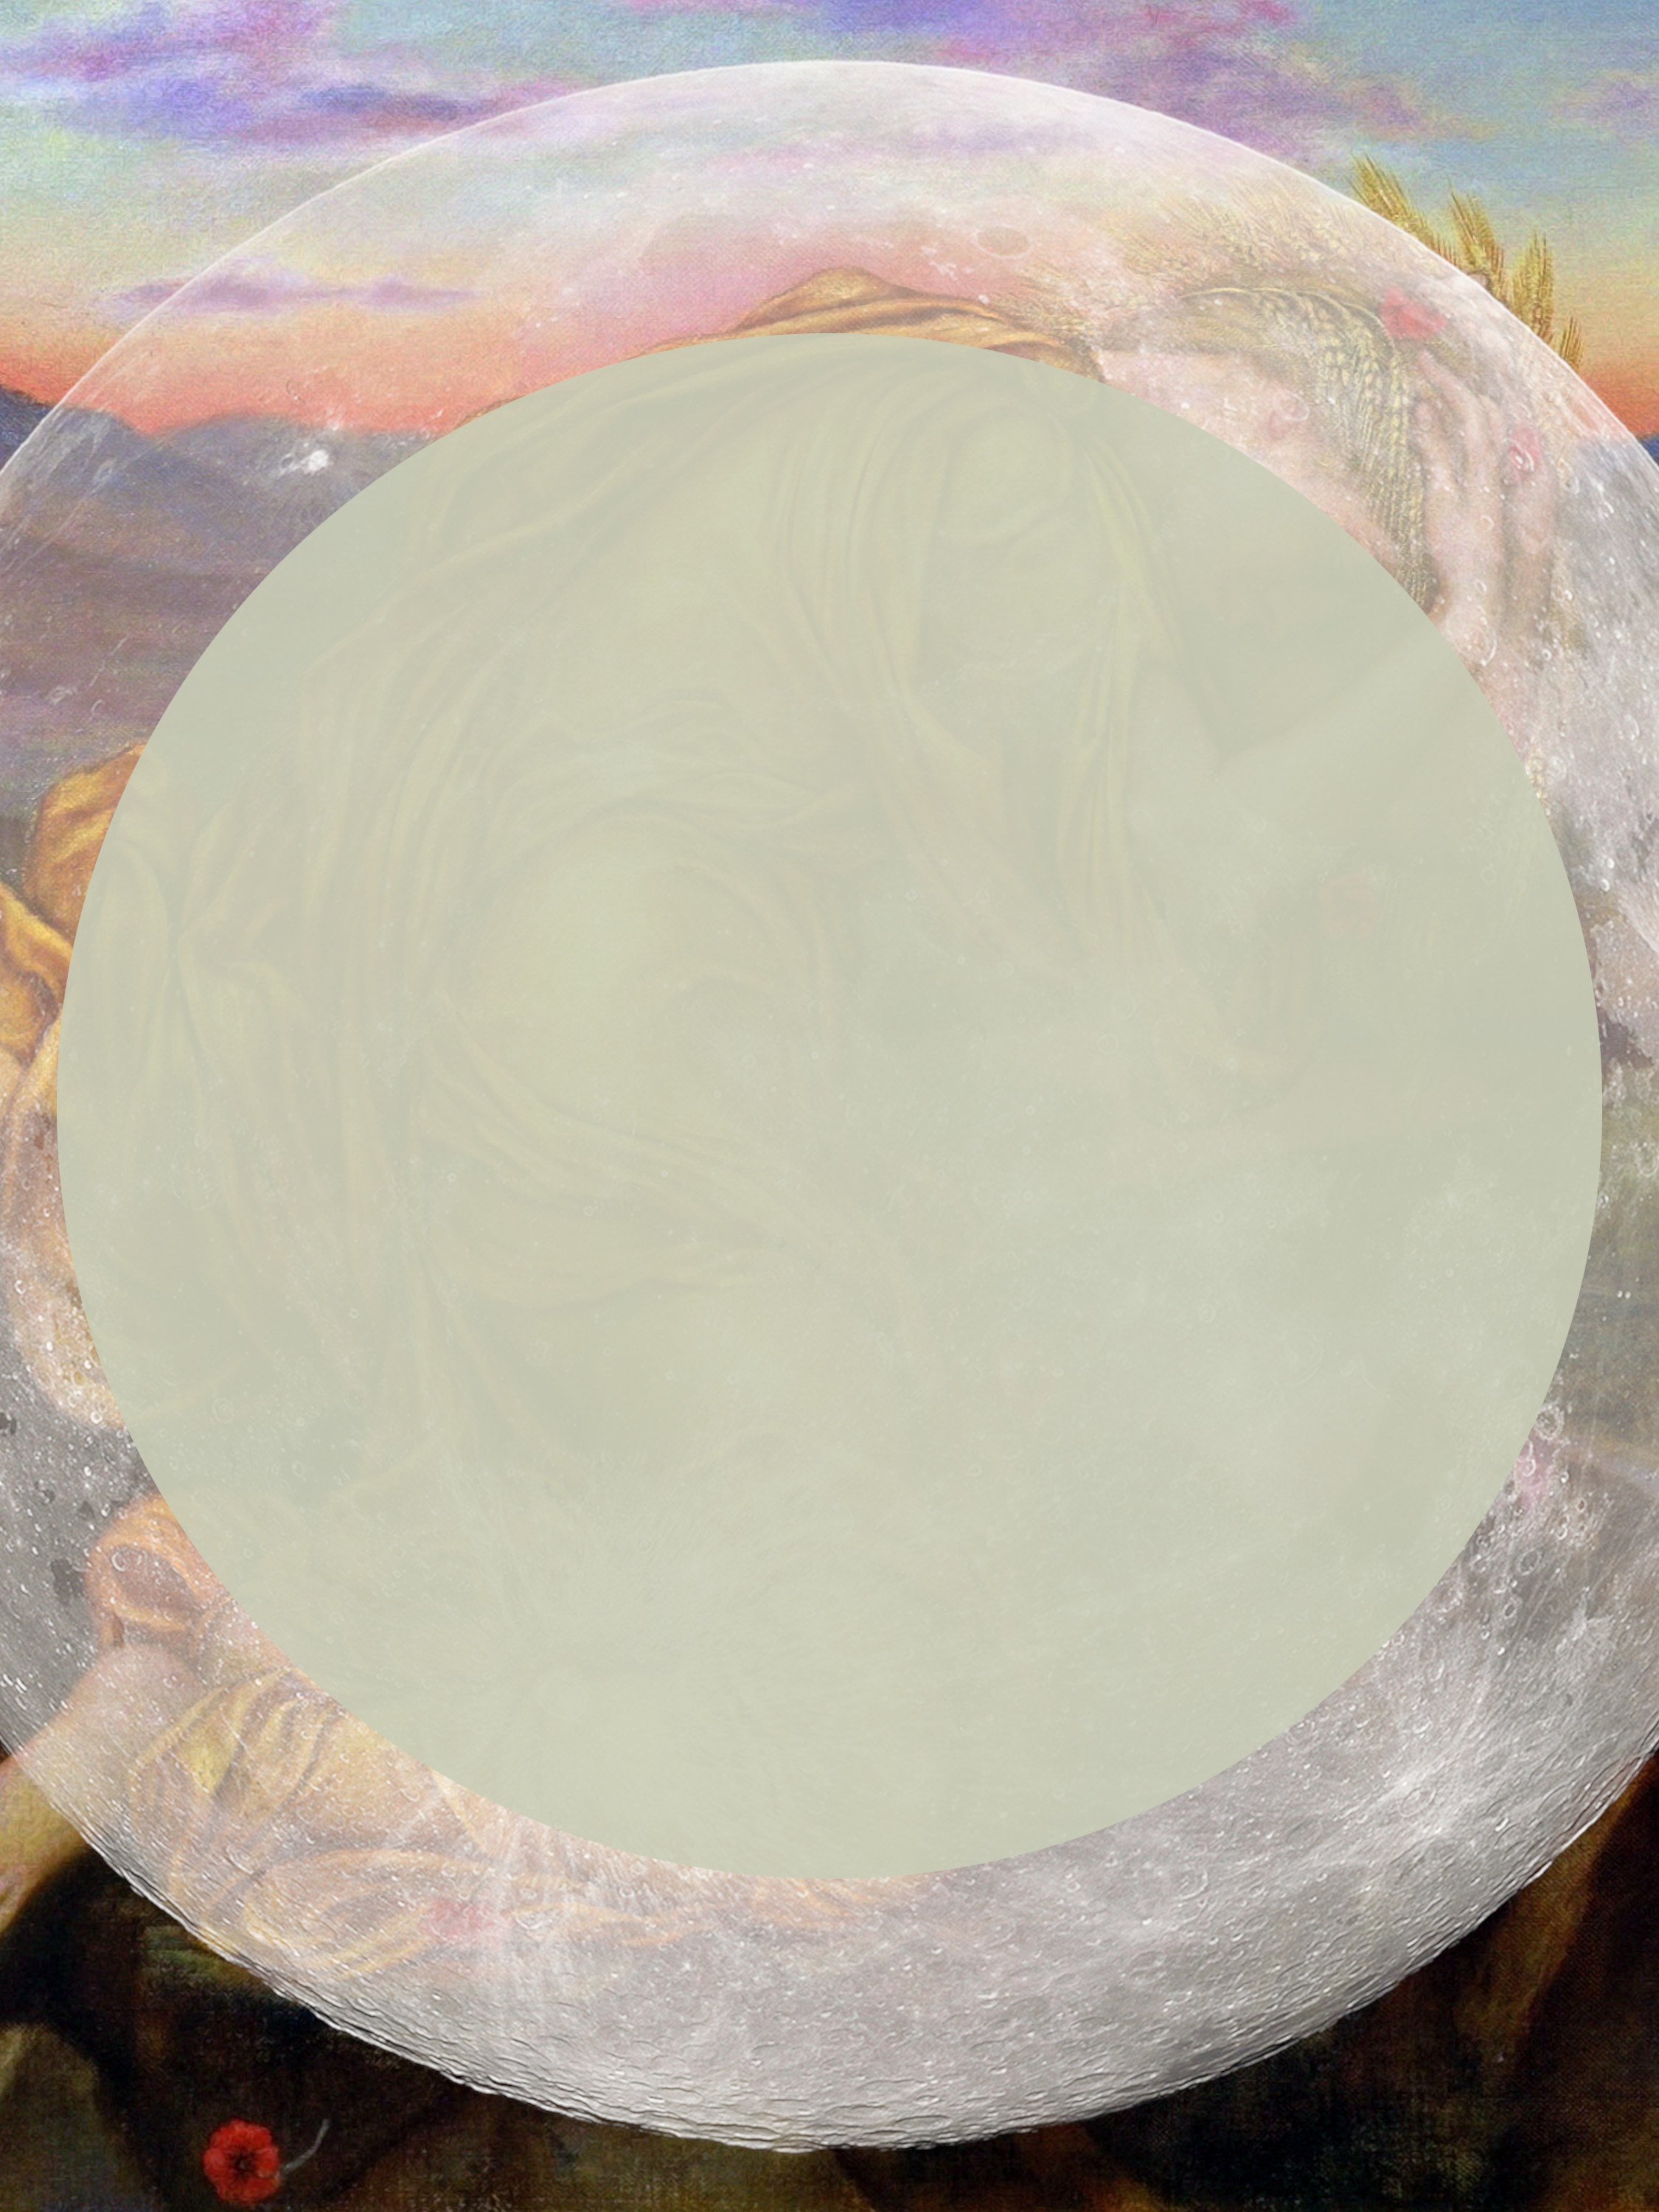
\includegraphics[width=\paperwidth,height=\paperheight]{moon5.jpeg}}
\begin{titlepage} % Suppresses headers and footers on the title page
	\centering % Centre everything on the title page
	%\scshape % Use small caps for all text on the title page

	%------------------------------------------------
	%	Title
	%------------------------------------------------

	\rule{\textwidth}{1.6pt}\vspace*{-\baselineskip}\vspace*{2pt} % Thick horizontal rule
	\rule{\textwidth}{0.4pt} % Thin horizontal rule
	
	\vspace{0.5\baselineskip} % Whitespace above the title
	
	{\scshape\Huge Plutarch \\ on the Face which appears on the Orb of the Moon}
	
	\vspace{0.5\baselineskip} % Whitespace above the title

	\rule{\textwidth}{0.4pt}\vspace*{-\baselineskip}\vspace{3.2pt} % Thin horizontal rule
	\rule{\textwidth}{1.6pt} % Thick horizontal rule
	
	\vspace{0.5\baselineskip} % Whitespace after the title block
	
	%------------------------------------------------
	%	Subtitle
	%------------------------------------------------
	
	{\scshape\small Translation and Notes, with Appendix \\ \Large
Arthur Octavius Prickard, \small M. A.}
 
        \vspace{0.25\baselineskip}
		
        {\scshape \small Formerly Fellow of New College, Oxford, and of Winchester College} % Subtitle or further description

	%------------------------------------------------
	%	Editor(s)
	%------------------------------------------------
        \vspace*{\fill}    

	\vspace{0.5\baselineskip}

	{\small\scshape London, 1911}
	
	{\small\scshape{Simpkin and Co., Ltd., Stationers Hall Court}}
	
	\vspace{0.25\baselineskip} % Whitespace after the title block

        {\scshape Internet Archive Online Edition}% Publication year}
    
	{\scshape\small Attribution NonCommercial ShareAlike 4.0 International } % Publisher
\end{titlepage}
\setlength{\parskip}{1mm plus1mm minus1mm}
\clearpage
\tableofcontents
\clearpage
\vspace*{\fill}
\begin{center}
``\emph{De ces deux infinis de nature, en grandeur et en petitesse, l'homme en conçoit plus aysément celui de grandeur que celui de petitesse.}'' --- Pascal.

\bigskip

``\emph{Look in the almanack, find out moonshine!}''
\end{center}
\vspace*{\fill}
\clearpage
\subsection*{Preface}
\paragraph{}
A few words of apology seem to be needed for the form in which this translation is presented. It was printed, without any idea of publication, in order to obtain a full revision by others, and to clear the ground for some further attempt to deal with the textual and other difficulties of this dialogue, before proceeding with other parts of Plutarch's \emph{Moralia}. As, however, it was clear that this revision could be better obtained if the draft were circulated more freely among a public, however limited, and as I was encouraged to think that the dialogue might interest some general readers, I decided to put it out as it stands, the printer adding some necessary aids, such as the insertion in the margin of the names of successive speakers. I have included notes on a few of the textual difficulties (to which my attention had been called by an eminent scholar, and which were my primary interest), and an introductory note calling attention to parts of the subject matter which seem to deserve the fuller consideration of competent persons. 

The text followed throughout has been that of Wyttenbach's Oxford edition. I have, I hope, called attention to every deviation from his readings, \emph{i. e.}, from those to be found in his text, or his translation, or his critical notes. I have derived much assistance from the Teubner edition throughout, and owe to it, in most cases, my first knowledge of modern corrections, including those of M. Bernardakis himself. As I have explained, I had not the materials for a continuous critical commentary. The few attempts which I have made at reconstruction may be thought somewhat hazardous; they might possibly seem less unjustifiable if the reader had before him the whole history of the text and of the corrections made by the great Renaissance scholars. I had entertained some hope that the severe nature of the subject matter, and the frequent references by Plutarch to older writers, might make it possible to proceed by way of hypothesis within fixed limits, and so to obtain a closer estimate of the general fidelity of the manuscripts which we have. However this may turn out, I have introduced no readings resting on hypothesis into the translation except in ch. 19, where an express reference to a passage of Aristotle seems to give a sure clue, and in ch. 26, where a rendering of αὐτοκράτορα (for παρακάτω) has slipped in almost by inadvertence.

Besides the unusually faulty state of the text, and its many \emph{lacunæ}, this dialogue is difficult because the ground is unbroken; there is no commentary. The notes of Wyttenbach on other parts of the \emph{Moralia} have been very helpful, and those of Holden on some of the \emph{Lives}. But for the most part, a reader or editor of the \emph{De Facie} must raise questions for himself, and then seek their solution. 

The special nature of the subject matter may be of help in dealing with the text; it brings in difficulties of its own. An excellent Spanish proverb, which I hope may be allowed to do service once again, will explain what I mean:--- ``It takes four men to make a salad; a spendthrift for the oil, a miser for the vinegar, a statesman for the salt, and a madman to stir.''\footnote{By the good offices of a friend I can give this in the original:--- ``Se necesitan cuatro para hacer una ensalada: un pródigo para el aceite, un avaro para el vinagre, un cuerdo para la sal y un loco para revolverla.'' --- From Diez, \emph{Dictionary of the Romance Languages}, I gather that ``loco'' is by etymology ``an owl.''} The Astronomer, the critical Scholar, and the philosopher, all have their rights in this dialogue ---
\begin{quotation}
``Three guests, I find, for different dishes call,

And how's one host to satisfy them all?''
\end{quotation}
\paragraph{}
Here the translator has been the guest, and the others the hosts. I have to acknowledge help generously and unsparingly given by several kind friends; if I do not name them, modesty is the cause, and not ingratitude. But there are limits to the advantageous use of the method of question and answer, which lie not in the patience of the experts consulted, but in the capacity of the questioner to put the right questions. Continuous co-operation may bring its own mischances, too. Failing the good fortune of some scholar who can speak familiarly the language of Science intervening, the ``madman'' must have the last hand in the dish.

I have specially mentioned two books which have been of the utmost service to me throughout: Kepler's annotated translation, the work of the last clouded years of a great life (though Plutarch's treatise had been an inspiration to him from an early time), and Dreyer's \emph{Planetary Systems}, to which I have often referred, but might properly have referred much oftener. Günther's translation of Kepler's ``Somnium'' (Leipzig, 1898), which does not include Plutarch's dialogue, has a full account of Kepler's work upon it, and some excellent diagrams. Ebner's Essay on the Geographical matter in Plutarch (Munich, 1906) is full of interest, and he, too, has closely studied Kepler.

In speaking of astronomical subjects, I have made no attempt to give explanations, being in no degree qualified to do so, except that I have attempted to realise, and convey to a reader, the conditions of knowledge under which Plutarch wrote. As it happened that a lunar eclipse took place while these sheets were being printed, I have availed myself of it to introduce a diagram prepared (roughly, no doubt) from the data contained in the ``Nautical Almanack'' of 1910. That printed on the cover is reproduced, by kind permission of Mr. R. Painton and the publishers of the \emph{English Mechanic and World of Science}, from their paper of November 25\textsuperscript{th}, 1910; it represents the moon shortly before totality on the night of the 16\textsuperscript{th}.

I have added a translation of Cicero's \emph{Somnium Scipionis}, partly because a second view of Astronomy in ancient literature seemed likely to round off and complete that given in Plutarch, partly from an uneasy feeling that the Stoics hardly received fair play in the \emph{De Facie}. At least they were sound on the Antipodes, and on a globular Earth. It is fortunate that they, and Latin literature also, can be represented by such a master of clear speech as this pupil of Poseidonius. And I have been fortunate in securing here the help of a very old friend, of whose Latinity I was as well assured as of his constant kindness; otherwise I might have shrunk from the attempt to render such a masterly specimen of the conversation of men whose ideal combined a ``leisure'' full of noble interests, with a ``dignity'' which was one thing with public duty.

Lastly, I hope that some indulgence may be accorded, if it should be necessary, to the ``loco'' who undertakes, even when helped by the best of printers, to be his own proof-reader.

\subsection*{Introductory Note}
\paragraph{}
The opening chapters of the Dialogue being lost, we have no clue to the place where it is supposed to take place, nor to the time --- unless one is given by the Eclipse of the Sun mentioned by Lucius in c. 19 --- and some points in the actual course of the discussion require a word of explanation. This can be most readily supplied by an enumeration of the speakers, in the order of their appearance, followed by a short analysis of the argument. Where the names are those of real persons living in Plutarch's lifetime, or of those who appear in other dialogues, I assume identity.

\subsection*{Persons of the Dialogue}
\paragraph{}
1. Sextius \emph{Sylla}, the Carthaginian, mentioned in the \emph{Life of Romulus} (c. 15) as ``a man wanting neither learning nor ingenuity,'' who had supplied Plutarch with a piece of archæological information. Elsewhere (\emph{De cohib. ira.} c. 1) he is addressed as ``O most eager Sylla!'' In another dialogue he declines to be led into a discussion on all cosmology by answering the question ``whether the egg or the bird comes first?'' (\emph{Quaest conv.} 2, 3).

He has a story, or myth, to tell about the Moon, which he is impatient to begin. This story, which he had heard from a friend in Carthage, is mainly geographical in interest. The details remind us of those quoted from Pytheas about his journeys to Britain and the Northern Seas. The whole conception of the globe is clearly earlier than that of Ptolemy (see especially as to the Caspian Sea, c. 26). The myth also introduces us to the worship of Cronus as practised at Carthage, and connects it with the wonders of the Moon, and her place in the heavenly system.

In c. 17 Sylla raises a good point, about the half-moon, which was being passed over.

2. \emph{Lamprias}, a brother, probably an elder brother, of Plutarch, who directs the course of the conversation, and himself expounds the Academic view, referring to Lucius for his recollections of a recent discussion at which both had been present, when the Stoic doctrines on physics had been criticised.

In some of the Symposiacs and other dialogues Lamprias takes a similar place; in others both brothers take part. Lamprias probably died early, see p. 15.

``Evidently a character, a good trencherman, as became a Boeotian, one who on occasion could dance the Pyrrhic war dance, who loved well a scoff and a jest ... and who, if he thrust himself somewhat brusquely into discussions which are going forward, was quite able to justify the intrusion.'' --- Archbishop Trench.

3. \emph{Apollonides}, astronomer and geometrician; perhaps the latter would be the more correct designation. In another dialogue (\emph{Quaest conv.} 3, 4) a ``tactician'' of the name appears.

As Apollonius, the great mathematician (living about 200 \textsc{bc}) was also a geometrician who contributed to astronomical theory, not himself an astronomer, it seems likely that the name Apollonides has been coined by Plutarch for ``one of the clan of Apollonius,'' \emph{i. e.}, a young professor of Geometry. Apollonius is treated rather brusquely by Lamprias, certainly with less respect than Menelaus. He seems to have cast in his lot with the Stoics in their physical opinions.

4. \emph{Aristotle}, a Peripatetic. Perhaps the name was given to him to mark the School to which he belonged. In the Dialogue ``On the deferred vengeance of the gods'' an ``Epicurus'' is a representative Epicurean.

5. \emph{Pharnaces}, a Stoic, who sturdily supports his physical creed against all comers.

6. \emph{Lucius}, an Etrurian pupil of Moderatus the Pythagorean, spoken of in one place (\emph{Quaest conv.} 8, 7 and 8) as ``Lucius our comrade.'' He is elsewhere reticent as to the inner Pythagorean teaching, but is courteous and ready to discuss ``what is probable and reasonable.''

Kepler is inclined to complain of his professorial tone and longwindedness in the present dialogue. This is hardly fair, as he is for the most part reporting a set discourse heard elsewhere, and that by request. Lamprias has to give him time to remember the points (c. 7). In c. 5 he asks that justice may be done to the Stoics. He associates himself with the Academics on physical matters.

7. \emph{Theon}, the Grammarian, represents literature (as he does in other dialogues, notably in that on the ``Ei at Delphi''). He is a welcome foil to the more severe disputants. In c. 24 he interrupts by moving the previous question --- ``Why a moon at all?'' and is congratulated on the cheerful turn which he has given to the discussion. He was Egyptian by birth. Theon may sometimes recall to readers of Jules Verne's pleasant \emph{Voyage autour de la lune} the sallies of Michel Ardan the Poet.

8. \emph{Menelaus}, a distinguished Astronomer who lived and observed at Alexandria. Observations of his, which include some taken in the first year of Trajan, \textsc{ad} 98, are recorded by Ptolemy (\emph{Magna Syntaxis} 7, 3, p. 170) and other writers.

\subsection*{Analysis}
\paragraph{}
[The opening chapters are lost. There must have been an introduction of the speakers, with some explanation as to time and place, a reference to a set discussion at which some of the speakers had been present, and a promise of Sylla to narrate a myth, bearing upon the Moon and her markings, which he had heard in Carthage. The conversation had taken a turn, prematurely as Sylla thinks, towards the mythical or supernatural aspects of the Moon.]

c. 1. It is agreed that the current scientific or quasi-scientific views on the markings of the Moon's face shall be first considered, then the supernatural.

cc. 2-4. Lamprias mentions
\begin{enumerate}
    \item The view that the markings are due to weakness of human eyesight. This is easily refuted.

    \item The view of Clearchus, the Peripatetic, that they are caused by reflexion of the Ocean on the Moon's face. But Ocean is continuous, the markings are broken; they are seen from all parts of the Earth, including Ocean itself (and the Earth is not a mere point in Space, but has dimensions of its own); and, thirdly, they are not seen on any other heavenly body.
\end{enumerate}
\paragraph{}
c. 3. The mention of Clearchus brings up the view, adopted from him by the Stoics, that the Moon is not a solid or earth-like body, but is fire or air, like the stars. This view had been severely handled in the former conference.

c. 6. Pharnaces complains that the Academics always criticise, never submit to be criticised. Let them first answer for their own paradox in confusing ``up'' and ``down,'' if they place a heavy body, such as the Moon is now said to be, above. Lucius retorts: ``Why not the Moon as well as the Earth, a larger body, yet poised in space?'' Pharnaces is unconvinced.

cc. 7-15. To give Lucius time to remember his points, Lamprias reviews the absurd consequences from the Stoic tenet that all weights converge towards the centre of our Earth. Why should not every heavy body, not Earth only, attract its parts towards its own centre? Again, if the Moon is a light fiery body, how do we find her placed near the Earth and immeasurably far from the Sun, planets and stars? How can we assume that Earth is the middle point of The Whole, that is, of Infinity? Lastly, allow that the Moon, if a heavy body, is out of her natural place. Yet why not? She may have been removed by force from the place naturally assigned to her to one which was better. Here the tone of the speaker rises as he lays down, often following the thought and the words of Plato's \emph{Timaeus}, the theory of creative ``Necessity'' and ``The Better.''

c. 16. Lucius is now ready to speak, but Aristotle intervenes with a reference to the view, held by his namesake, that the stars are composed of something essentially different from the four elements, and that their motion is naturally circular, not up or down. Lucius points out that it is degrading to the Moon to call her a star, being inferior to the stars in lustre and speed, and deriving her light from the Sun. For this, the view of Anaxagoras and of Empedocles, is the only one consistent with her phases as we see them (not that quoted from Poseidonius the Stoic).

c. 17. To an enquiry from Sylla whether the difficulty of the half-moon (\emph{i. e.} how does reflexion, being at equal angles, then carry sunlight to the Earth, and not off into space beyond us?) had been met, Lucius answers that it had. The answer given was: \emph{1.} Reflexion at equal angles is not a law universally admitted or true; \emph{2.} there may be cross lights and a complex illumination; \emph{3.} it may be shewn by a diagram (though this could not be done at the time) that some rays would reach the earth; \emph{4.} the difficulty arises at other phases also. He repeats the argument drawn from the phases as we see them; and ends with an analogy: Sunlight acts on the Moon as it does on the Earth, not as on the air; therefore the Moon resembles Earth rather than air.

c. 19. This is well received, and Lucius refers (a second analogy) to Solar Eclipses, and in particular to a recent one, to shew that the Moon, like the Earth, can intercept the Sun's light, and is therefore, like it, a solid body. The fact that the track of the shadow is narrow in a solar eclipse is explained from the figures and distances.

c. 20. Lucius continues his report, and describes in detail what happens in a lunar eclipse. If the Moon, he concludes, were fiery and luminous, we should only see her at eclipse times, \emph{i. e.} at intervals normally of six months, occasionally of five.

c. 21. Pharnaces and Apollonides both rise to speak. Apollonides raises a verbal point about the word ``shadow''; Pharnaces observes that the Moon does shew a blurred and fiery appearance during an Eclipse, to which Lamprias replies by enumerating the successive colours of the Moon's face during Eclipse, that proper to herself being dark and earth-like, not fiery. He concludes that the Moon is like our Earth, with a surface broken into heights and gullies, which are the cause of the markings.

c. 22. Apollonides objects that there can be no clefts on the moon with sides high enough to cast such shadows. Lamprias replies that it is the distance and position of the light which matter, not the size of objects which break it; 

c. 23. And goes on himself to supply a stronger objection --- that we do not see the Sun's image in the Moon --- and the answer. This is twofold \emph{a.} general, the two cases differ in all details \emph{b.} personal to those who, like himself, believe the Moon to be an earth, and to have a rough surface. Why should we see the Sun mirrored in the Moon, and not terrestrial objects or stars?

c. 24. Sylla's myth is now called for, and the company sits down to hear it. But Theon interposes: Can the Moon have inhabitants or support any life, animal or vegetable? If not, how is she ``an earth,'' and what is her use?

c. 25. Theon's sally is taken in good part, and gravely answered at some length by Lamprias.

c. 26. The mention of life on the Moon calls up Sylla, who again feels that he has been anticipated. He begins his myth, heard from a stranger met in Carthage, who had himself made the northward voyage and returned. Once in every thirty years (or year of the planet Saturn) an expedition is sent out from Carthage to certain islands in the Northern Atlantic where Cronus (Saturn) reigns in banishment. The stranger had charged Sylla to pay special honour to the Moon, 

cc. 27-29. instructing him as to the functions of Persephone in bringing about the second death --- the separation of mind from soul --- which takes place on the Moon, and the genesis of ``Daemons,''

c. 30. to whom are assigned certain functions on Earth. Sylla commends the myth to his hearers.

\bigskip
\centerline{\EightStarTaper}
\centerline{\EightStarTaper\EightStarTaper}
\bigskip

The dialogue ``On the Face in the Moon'' is not a scientific treatise, and its author would have disclaimed any intention of writing for scientific men. It is discussion for the sake of discussion, the ``good talk'' of which Plutarch wished that Athens should have no monopoly in his own day, any more than it had when the Boeotian Simmias and Cebes were numbered among the most trusty friends of Socrates, or, later, when ``plain living and high thinking'' could be exhibited in lofty perfection in the Theban home of Epaminondas. A mixed company, including an astronomer, another mathematician, a literary man, and professed philosophers, with Plutarch's brother, Lamprias, a genial and sensible president, discusses the movements and nature of the Moon from many points of view. That the weightiest part of their arguments consists in an assault on the Stoic view that the Moon is a fiery or starlike body, and no earth, will not surprise us if we remember that the Stoics were used to such attacks; no one denounced their physical absurdities (drawn from Aristotle, perversely followed) more roundly than the Stoics themselves, notably Seneca. (See \emph{Physical Science in the time of Nero}, by Clarke and Geikie; Macmillan, 1910.) The interest in natural phenomena which Plutarch shows throughout the ``Lives,'' touched by a still greater interest in their bearing on men and life, and coloured by an eye ready to see what was picturesque or ludicrous in them, makes him a pleasant, and, with certain reservations, a competent reporter. Like our own Sir Thomas Browne, though without his training or scientific grasp, he had a good deal of sympathy with mystical and occult explanations; and he shows a constant desire to mediate between ``Superstition'' and ``Atheism.''

It happens that this dialogue might, if carefully examined, yield material of some importance for the history of Greek science. It must have been written not very long --- say a generation --- before Ptolemy's standard book, the \emph{Magna Syntaxis}, but it contains no reference to him, and shows no consciousness of his views and work. Now Ptolemy is almost our only authority as to the discoveries of Hipparchus, the ``Father of Astronomy,'' who lived some three hundred years before him. It is often difficult to be sure from his language how much is to be credited to himself, and how much to Hipparchus. Delambre is always inclined to disparage the originality of Ptolemy, and De Morgan often questions Delambre's conclusions. (See Art. Cl. Ptolemaeus, in Smith's \emph{Dict. Biog.}, also the \emph{Penny Cyclopædia}.) There were workers of importance in the interval, such as the great mathematician Apollonius, and the Stoic Poseidonius, though no first-rate astronomer. Thus a lively account of the state of science in Plutarch's time, so far as it could be made intelligible to an educated company, should have its value. 

Here we will only attempt to collect a few instances which illustrate Plutarch's way of dealing with these subjects, as it strikes an ordinary reader.

\emph{1.} In c. 20, in order to account for the fact that the Moon is first eclipsed on her eastern side, the Sun on his western, it is stated that the shadow of the earth moves from East to West, the Sun and the Moon from West to East, so that the Sun is overtaken by the shadow of the Moon, but the Moon meets that of the earth. Really, all three move (speaking geocentrically, though this makes no essential difference) from West to East; in both the cases the Moon, travelling some twelve times as fast as the Sun, overtakes him, or the earth's shadow thrown by him; in one she is the darkening, in the other the darkened body. The statement is put into the mouth of Lucius, who, after reporting the chief arguments used by ``Our Comrade'' in the previous discussion, adds some points of his own. The view may be one hastily formed by the Author on a matter where confusion is easy; it can hardly have reached him from a professional source.

\emph{2.} Lucius mentions, as another additional point, ``the duration and magnitude of lunar eclipses.''

``If she is eclipsed when high up and far from the earth, she is hidden for a short time; if when near the earth and low down, she is firmly held and emerges slowly out of the shadow; and yet when she is low her speed is greatest, when high it is least.''

Kepler demurs to the fact, and says that, in his experience, Perigee eclipses are the shorter; this must be understood \emph{ceteris paribus}, since the precise conditions of no two eclipses, at least within a very long cycle of years, are the same. The last words of Lucius state correctly the second of two conflicting conditions. The shadow cone to be crossed will be broadest when the Moon is near the Earth, but she travels more slowly when distant, in accordance with the principle afterwards embodied in Kepler's \emph{Second Law}. When the two conditions are stated in figures, it seems that \emph{ceteris paribus} an eclipse of a distant Moon should be the longer by about one fifteenth. Kepler suggests a scientific reason for the mistake, so far as there is any. Was Plutarch also led by his own picturesque conception of the Moon struggling through the lower circles of the cone, to prefer, where views were evenly balanced, the one most consistent with it?

\emph{3.} The figures given in c. 20 raise a question. ``Out of the 465 occurrences of full Moon at eclipse intervals, 404 show an interval of six months, the remainder one of five.'' The numbers correspond correctly to the lunar eclipses of a little over 220 years. In that time there would be twelve recurrences of the cycle first known to the Greeks from Oriental astronomers, and called the Saros, each cycle being 223 lunar months or 18 years 11 days, in all 216 years 132 days. This total will account for 60 five-month eclipses and 396 six months opportunities (268 actual eclipses), and about four years more to one five-months eclipse and eight opportunities, so that the totals for 220 years will be those given in the text. But what was this period which included ``\emph{the} 465 etc.''? It does not seem to be mentioned elsewhere?

\emph{4.} In c. 17 reference is made to the optics of ``folding mirrors,'' \emph{i. e.}, plane mirrors placed at an angle (\emph{i. e.}, an angle of 60° in the case mentioned) to one another. We are told that the cause is given by Plato. But the words quoted from Plato (Timaeus, c. 16, p. 46 C.) are used to explain reflexion from concave mirrors, and it is difficult to give them a meaning as applied by Plutarch. However, there is confusion and repetition in our text, and concave mirrors are mentioned above.

\emph{5.} The language used in chapters 24 and 25 (often highly technical) as to the Moon's movements and the Epicyclic Theory, appears to refer to current controversies, settled later on by Ptolemy, and to deserve careful examination by a competent critic.

The Dialogue which suggests these questions may well be more instructive to us than a more professional treatise could be. Astronomy had, in its proper course of development, become very technical and mathematical, sharply distinguished from general physical enquiry. Even Hipparchus, we are told, ``though he loved truth above everything,'' yet was not versed in ``natural science,'' and was content to explain the motions of the heavenly bodies by an hypothesis mathematically consistent, without care for its physical truth (see Dreyer, p. 165, and the passages quoted from Theon of Alexandria and Ptolemy). Take the case of the Moon. Ptolemy was content to ``save the phenomena,'' to borrow a favourite phrase, by a system which admirably accounted for her very complex movements, but which involved the consequence that her distance from us at the nearest must he half that at the farthest, and her angular diameter therefore double!

One bold thinker of earlier times, when an astronomer might concern himself also with physical facts, is twice mentioned. It will not be beside our purpose to look into his two great efforts, one of calculation, one of theory.

We read in c. 10 that ``Aristarchus in his book on \emph{Magnitudes and Distances} shows that the distance of the Sun is more than eighteen times that of the Moon, and less than twenty times.'' The book is extant (ed. Wallis, Oxford, 1688), and the process seems to be as unexceptionable in theory as it was audacious. Aristarchus set himself to catch the moment of half-moon, and in the right-angled triangle Sun --- Moon --- Earth, to determine the large angle at Earth. This he found to be 29/30 of a right angle, or 87°, whereas it is really (theoretically, at least) 89° 50$^{\prime}$. This was harmless enough, but it involved a large relative error in the small angle, Earth --- Sun --- Moon, which became 3° instead of 10$^{\prime}$, eighteen times too much. The sequel is very interesting. Hipparchus, a century later, adopted this result in his calculation of the parallax (angle subtending the earth's radius) of the Sun, which he found to be 3$^{\prime}$ (twenty times too much). This was adopted by Ptolemy in the second century \textsc{ad}, and remained the official estimate until nearly 1700 \textsc{ad}, though both Hipparchus and Kepler protested, the latter stating as his opinion that the parallax could not be greater than one minute of arc, or the distance less than twelve millions of miles. Shortly before 1700 \textsc{ad} improved knowledge of the orbit and distances of Mars enabled the Sun's parallax to be reduced to 9 1/2 seconds of arc. Lastly, Halley, Savilian Professor of Geometry at Oxford, and also Astronomer Royal, had the splendid privilege of pointing out the method which he had no chance of practising himself, but which has since been repeatedly applied, though to some extent superseded,\footnote{See Turner's \emph{Modern Astronomy}, p. 95 foll.} the current settlement (a little under 9 seconds of arc) dating from 1867. It was a great achievement of Aristarchus, though he misled the world for so many centuries, to state a figure at all, and to think in such mighty units. Perhaps the attempt could not have been made in a more advanced state of his science.

His cosmical speculation is even more daring. It is known to us from this dialogue (c. 6) and also from the great mathematician and engineer Archimedes of Syracuse (born about 287 \textsc{bc}), who records it (in his extant \emph{Arenarius}) without comment on the main point. Aristarchus proposed to ``disturb the hearth of the universe'' by his hypothesis that the heaven of the stars is fixed, while the earth has a daily motion on her axis and an annual motion round the sun. It was a brilliant intuition, possible in an age of comparatively simple knowledge, which could not easily have been made when the complexity of the several orbits was increasingly realised (see Dreyer, pp. 147-8). If we may, without irreverence, use an analogy, it was like the happy efforts which novices often make in an exercise requiring skill of mind or body, relapsing into incompetence when the technical conditions are better understood. Dr. Dreyer (p. 145) makes the interesting suggestion that Aristarchus took the idea from some early form of the system of ``movable excentrics,'' and further (p. 157), that if that system had, in later times, prevailed against that of Epicycles, its rival in displacing the cumbrous ``concentric spheres'' known to Aristotle, it must have flashed, sooner or later, upon some bright mind, that there was one excentric point, namely, in the Sun, central to the orbits of all the planets. It is as tempting as it is idle to speculate on what might have happened if a heliocentric view had been stereotyped by Ptolemy and Thomas Aquinas, and the geocentric abandoned to a few heretics and a few great lagging minds, as Francis Bacon and Sir Thomas Browne did lag later on. To Ptolemy the question would hardly be of the first interest. The ``phenomena'' of the Solar system are ``saved'' perfectly well on either hypothesis. And until people became familiar with the conception of one law for all matter in space, the actual movements remained of little concern.

Kepler (\emph{Epit. Astron. Copern.}, 4) remarks that in stating the uses of the Moon (c. 25) Lamprias has made an omission :--- she gives man a means of approach to the planetary system. No one could speak with more absolute authority on this particular point, but we may give some details suggested by Plutarch's dialogue. From her apparent size, her nearness, the frequent recurrence of her phases, it was obvious that man should first turn to our nearest neighbour. There was the further advantage that, in all early stages of lunar enquiry, it was quite indifferent whether the sun turns round the earth, or the earth round the sun, or both round a common centre. Whether the Greeks owed much or little to the East, they soon came to realise that the moon really moved round the earth at a moderate distance, as the nave of a wheel round the axle. Soon it appeared that there were irregularities in this circular movement. The ``First Anomaly,'' a difference in speed at various parts of the orbit, was well understood by Hipparchus and Ptolemy, and at last interpreted by Kepler as due to the fact that the orbit is, approximately, an ellipse not a circle (not apparently till \emph{after} he had solved the difficult orbit of Mars). Finally, that a body thus revolving round another must move in an ellipse, with the larger body in one focus, was settled by Newton. The ``Second Anomaly'' was indicated by Hipparchus, fully worked out by Ptolemy, and known as ``the Evection'' to more modern times, its cause, namely the interference of a third body, the sun, being again first explained by Newton. Other difficult points in the moon's movement, as the inclination of her orbit to that of the sun (earth), and the retrogression of the points of intersection of the two orbits, were familiar to Hipparchus. A third ``Anomaly,'' now known as ``Variation,'' is instructive, because its discovery has been claimed for an Arabian astronomer, of about 1000 \textsc{ad} After an exhaustive discussion during the last century (1836-1871), it seems proved that the claim rested upon a mistake, and that the sole credit is due to Tycho Brahe (1598). (See Dreyer, p. 252.)

Turning from the movements to the physical aspects of the moon, we find from Plutarch that very correct ideas prevailed as to her size, distance, and the composition of her crust; and it was at least guessed that her density was less than that of the earth. On the other hand, she was erroneously supposed to share with us an atmosphere, in which comets move. Of great and far-reaching interest is the opinion which we find advanced, that earth and moon attract, each from its own centre, their own parts; and that if the earth draws the moon, it is as a former part of itself, just as it attracts back a stone which is thrown upwards (see too Dreyer, p. 189). The moon is a sphere, always presenting the same face to the earth. There is no suggestion of rotation on an axis; indeed this appears to be expressly excluded.

It may cause a smile, on first reading, to find the earth-like nature of the moon, and similar truths, treated as open to argument. But our superior enlightenment is really very modern. Bacon gives a grudging assent to the new doctrine that the moon may be a body like the earth, but declines to extend it to other bodies in the heavens, and says that his own theory is against it. Sir Thomas Browne reserves for discussion the question: ``Whether the globe of the earth be but a point in respect of the stars and firmament,'' and Galileo writes to Muti in 1616: ``I said then and I say now that I do not believe that the body of the moon is composed of earth and water ... I added further: Even allowing that the matter of the moon may be like that of the earth (a most improbable supposition) still not one of those things that the earth produces can exist on the moon.'' Much has been said and written since --- and the moon keeps her countenance!

Daniel Ruhnken, in his Inaugural Lecture (\textsc{ad} 1757) \emph{De Græcia artium ac doctrinarum inventrice}, an eloquent and weighty survey, warns us against a certain childishness in any comparison between ancient and modern astronomy, and lays stress upon the gains in actual knowledge and in increased accuracy due to instruments. The case, so far as instruments are concerned, is much stronger now than it was thirty years after Newton's death, but perhaps the essential points are the same, and are two. There is first the aim of the modern astronomer, which is to account for the position in space of the heavenly bodies; and, secondly, the mathematical conceptions, which are his best instruments, are of an order altogether higher. There has been continuity, but there has also been advance \emph{per saltum}. If Xerxes had won at Salamis, and had succeeded in sterilising the genius of the Hellenic race, the giants of the Revival in Europe, in which the Hellenic spirit was only one factor, would surely have made up the missing ground, but there would have been much to make up before the advance went on. These great things apart, it is interesting to trace the early glimmerings, sometimes fanned into brightness, and to follow the ``good talk'' of a party meeting in Boeotia perhaps late in the first century \textsc{ad} about the ``Face in the Moon'' and all that it meant. Horace, a century earlier, compares the Greek genius of his day to a little girl in the nursery --- ``What she sought eagerly she soon tired of and let be'' --- a sad estimate for those who remember what Greece at her best has done for us, and all the more sad, because it was deliberate and unbiassed. It is consoling to find, in one branch of enquiry, so much steadiness of purpose and persevering effort, every step an advance, and scarcely one which needed to be recalled; continuous advance from Thales to Ptolemy and the later Theon. That no new contribution came from any other quarter, from the learned Romans or Indians or Arabians, until the birth of the new order, need not be matter of boasting; it is simple fact.

Plutarch was born about 50 \textsc{ad} at Chaeroneia in Boeotia, and was living at least as late as 115 \textsc{ad} We have little information as to the dates of his several works. M. Gréard (p. 45) thinks that all the Lamprias dialogues, of which this is one, are early in date, and that Lamprias himself died young. We have a clue to the date of this dialogue in the recent Solar Eclipse mentioned in c. 19, which would help us more if we knew the place where the eclipse was observed; we should naturally assume this to have been in Boeotia. Various eclipses have been examined by modern authorities; see the special note.

It would be out of place, in connexion with the dialogue before us, to speak at any length on Plutarch's life, or of his characteristics as a man, a stylist, and a moralist. On all these points a reader may be referred to the excellent ``lives'' by Dryden or Dacier, to the small volume of lectures by Archbishop Trench, to chapters in Mr. Dill's \emph{Roman Society Nero to Aurelius}, and in Mr. Glover's recent \emph{Conflict of Religions}, and to pages, all too few, in the late Dr. C. Bigg's works; and to the very beautiful and careful study by M. Octave Gréard. The style causes some difficulty to a translator, since it would be unfaithful to the Author to represent it by clear and unencumbered periods. But it is a very honest style; Plutarch, though steeped in Plato, never attempts to write with Plato's pen; and the man is always apparent in the style. I have made free use of Amyot's version, which combines faithfulness with ease in a degree which may well make those who follow him despair.\footnote{See, however, Gréard, p. 358 foll.} As a physicist, Plutarch was genuinely interested both in mathematics (Sympos., 9, 14, etc.), and in natural phenomena; but his tastes were too miscellaneous for accuracy to be possible. Indeed he makes no pretence to accuracy; but no one dreams of his reputation suffering on that account, and he puts accuracy out of fashion with his readers. He was not a philosopher (Glover, p. 89), but he knew a vast deal about philosophers. In the \emph{De Facie} it is sometimes amusing, and sometimes irritating, to watch the superior tone which the Academic speakers are allowed to assume in questioning or contradicting the scientific men present. As a practical moralist, with a strong vein of mysticism, Plutarch stands alone. It was the latter quality which gave him his strong interest in the moon, closely connected as she was with the mysteries of birth and death, and with the Spirits, or Genii, who help the endeavours of men on earth, and minister to their needs. But he was the practical moralist above all things, and would have endorsed, as a sane and lofty utterance, the words of the unhappy astronomer in \emph{Rasselas}:--- ``\emph{To man is permitted the contemplation of the skies, but the practice of virtue is commanded.}''\footnote{There is a short word, τῦφος, often used by Plutarch, and always difficult to translate, which may be interpreted through its associates. It is coupled with Superstition (δεισιδαιμονία), Opinionativeness (οἴημα), Stupidity (ἀβελτερία), Pretentiousness (σεμνότης), Desire of applause (8o£δοξοκοπία), and other unlovely qualities. We cannot draw a man's character by merely summing up his antipathies, but the enumeration may help us to understand Plutarch's attitude, at once robust and finely sympathetic, towards men and their opinions.}
\clearpage
\section{On the Face which appears on the Orb of the Moon}
\paragraph{}
C. --- 1. Here Sylla said: ``Enough of all this, for it belongs to my story, and comes out of it. But I should like to ask in the first place whether we are to have a prelude, and first to discuss those views about the Moon's face which are in everyone's hand and on everyone's lips.'' ``Of course we are,'' I answered, ``it was the difficulty which we found in these which thrust us upon the others. In chronic diseases, patients grow weary of the common remedies and plans of treatment, and turn to rites and charms and dreams. Just so in obscure and perplexing enquiries, when the common, received, familiar accounts are not convincing, we cannot but try those which lie further afield; we must not despise them, but simply repeat the spells which the old people used, and out of it all try to elicit the truth.

2. ``To begin, you see the absurdity of calling the figure which appears in the Moon an affection of our eyesight, too weak to resist the brightness, or, as we say, dazzled; and of not observing that this ought rather to happen when we look at the Sun, who meets us with his fierce strong strokes. Empedocles\footnote{For quotations from early philosophers see Diels' ``Fragmenta'' (1901, etc.), also ``Heracliti Reliquiæ'' (Bywater, 1877), and other special collections.} has a pretty line giving the difference between the two:---
\begin{quotation}
`The Sun's keen shafts, and Moon with kindly beams.'
\end{quotation}
\paragraph{}
Thus he describes the attractive, cheerful, painless quality of her light. Further, the reason is given why men of dim and weak eyesight do not see any distinct figure in the moon; her orb shines full and smooth to them, whereas strong-sighted persons get more details, and distinguish the features impressed there with clearer sense of contrast. Surely, the reverse should happen if it were a weakness and affection of the eye which produced the image; the weaker the organ the clearer should be the appearance. The very irregularity of the surface is sufficient to refute this theory; this image is not one of continuous and confluent shadow, but is well sketched in the words of Agesianax:---
\begin{quotation}
`All round as fire she shines, but in her midst,

Bluer than cyanus, lo, a maiden's eye,

Her tender brow, her face in counterpart.'
\end{quotation}
\paragraph{}
For the shadowy parts really pass beneath the bright ones which they encircle, and in turn are caught and cut off by them; thus light and shade are interwoven throughout, and the face-form is delineated to the life. The argument was thought to meet your Clearchus also, Aristotle, no less unanswerably; for yours he is, and an intimate of your namesake of old, although he perverted many doctrines of The Path.''

3. Here Apollonides interposed to ask what the view of Clearchus was. ``No man,'' I said, ``has less good right than you to ignorance of a doctrine which starts from Geometry, as from its own native hearth. Clearchus says that the face, as we call it, is made up of images of the great ocean mirrored in the Moon. For our sight being reflected back from many points, is able to touch objects which are not in its direct line; and the full moon is of all mirrors the most beautiful and the purest in uniformity and lustre. As then you geometers think that the rainbow is seen in the cloud when it has acquired a moist and smooth consistence, because our vision is reflected on to the sun, so Clearchus held that the outer Ocean is seen in the moon, not where it really is, but in the place from which reflexion carried our sight into contact with it and its dazzle.\footnote{Ar. Probl. 12, 3.} Agesianax has another passage:---
\begin{quotation}
`Or Ocean's wave that foams right opposite,

Be mirrored like a sheet of fire and flame.' ''
\end{quotation}
\paragraph{}
4. This pleased Apollonides. ``What a fresh way of putting a view; that was a bold man, and there was poetry in him. But how did the refutation proceed on your side?'' ``In this way,'' I answered. ``First the outer Ocean is uniform, a sea with one continuous stream, whereas the appearance of the dark places in the moon is not uniform; there are isthmuses, so to call them, where the brightness parts and defines the shadow; each region is marked off and has its proper boundary, and so the places where light and shade meet assume the appearance of height and depth, and represent quite naturally human eyes and lips. Either, therefore, we must assume that there are more oceans than one, parted by real isthmuses and mainlands, which is absurd and untrue; or, if there is only one, it is impossible to believe that its image could appear thus broken up. Now comes a question which it is safer to ask in your presence than it is to state an answer. Given that the habitable world is `equal in breadth and length,' is it possible that the view of the sea as a whole, thus reflected from the moon, should reach those sailing upon the great sea itself, yes, or living on it as the Britons do, and this even if the earth does, as you say it does, occupy a point central to the sphere of the moon? This,'' I continued, ``is a matter for you to consider, but the reflexion of vision from the moon is a further question which it is not for you to decide, nor yet for Hipparchus. I know, my dear friend [that Hipparchus is a very great astronomer], but many people do not accept his view on the physical nature of vision, that it is probably a sympathetic blending and commixture, rather than a succession of strokes and recoils such as Epicurus devised for his atoms. Nor will you find Clearchus ready to assume that the moon is a weighty and solid body. Yet `an ethereal and luminous star,' to use your words, ought to break and divert the vision, so there is no question of reflexion. Lastly, if anyone requires us to do so, we will put the question, how is it that only one face is seen, the sea mirrored on the moon, and none in any of all the other stars? Yet reason demands that our vision should be thus affected in the case of all or of none. But now,'' I said, turning to Lucius, ``remind us which of our points was mentioned first.''

5. ``No,'' said Lucius; ``to avoid the appearance of merely insulting Pharnaces, if we pass over the Stoic view without a word of greeting, do give some answer to Clearchus, and his assumption that the moon is a mere mixture of air and mild fire, that the air grows dark on its surface, as a ripple courses over a calm sea, and so the appearance of a face is produced.''

``It is kind of you, Lucius,'' I said, ``to clothe this absurdity in sounding terms. That is not how our comrade dealt with it. He said the truth, that it is a slap in the face to the moon when they fill her with smuts and blacks, addressing her in one breath as Artemis and Athena, and in the very same describing a caked compound of murky air and charcoal fire, with no kindling or light of its own, a nondescript body smoking and charred like those thunderbolts which poets address as `lightless' and `sooty.' That a charcoal fire, such as this school makes out the moon to be, has no stability or consistence at all, unless it find solid fuel at once to support and to feed it, is a point not so clearly seen by some philosophers as it is by those who tell us in jest that Hephaestus has been called lame because fire advances no better without wood than lame people without a stick! If then the moon is fire, whence has it all this air inside it? For this upper region, always in circular motion, belongs not to air but to some nobler substance, which has the property of refining and kindling all things. If air has been generated, how is it that it has not been vaporised by the fire and passed away into some other form, but is preserved near the fire all this time, like a nail fitted into the same place and wedged there for ever? If it is rare and diffused, it should not remain stable, but be displaced. On the other hand, it cannot subsist in a solidified form, because it is mingled with fire, and has no moisture with it nor yet earth, the only agents by which air can be compacted. Again, rapid motion fires the air which is contained in stones, and even in cold lead, much more than that which is in fire, when whirled round with such velocity. For they are displeased with Empedocles, when he describes the moon as a mass of air frozen like hail and enclosed within her globe of fire. Yet they themselves hold that the moon is a globe of fire which encloses air variously distributed, and this though they do not allow that she has clefts in herself, or depths and hollows, for which those who make her an earth-like body find room, but clearly suppose that the air lies upon her convex surface. That it should do so is absurd in point of stability, and impossible in view of what we see at full moon; for we ought not to be able to distinguish black parts and shadow then; either all should be dull and shrouded, or all should shine out together when the moon is caught by the sun. For look at our earth; the air which lies in her depths and hollows, where no ray penetrates, remains in shadow unilluminated; that which is outside, diffused over the earth, has light and brilliant colouring, because from its rarety it easily mingles, and takes up any quality or influence. By light, in particular, if merely touched, or, in your words, grazed, it is changed all through and illumined. This is at once an excellent ally to those who thrust the air into depths and gullies on the moon, and also quite disposes of you, who strangely compound her globe of air and fire. For it is impossible that shadow should be left on her surface when the sun touches with his light all the moon within our own field of vision.''

6. Here Pharnaces, while I was still speaking, broke in: ``There it is again, the old trick of the Academy brought out against us; they amuse themselves with arguing against other people, but in no case submit to be examined on their own views, they treat their opponents as apologists, not accusers. I can speak for myself at any rate; you are not going to draw me on today to answer your charges against the Stoics, unless we first get an account of your conduct in turning the universe upside down.'' Lucius smiled: ``Yes, my friend,'' he said, ``only do not threaten us with the writ of heresy, such as Cleanthes used to think that the Greeks should have had served upon Aristarchus of Samos, for shifting the hearth of the Universe, because that great man attempted `to save phenomena' with his hypothesis that the heavens are stationary, while our earth moves round in an oblique orbit, at the same time whirling about her own axis. We Academics have no view of our own finding, but do tell me this --- why are those who assume that the moon is an earth turning things upside down, any more than you who fix the earth where she is, suspended in mid-air, a body considerably larger than the moon? At least mathematicians tell us so, calculating the magnitude of the obscuring body from what takes place in eclipses, and from the passages of the moon through the shadow. For the shadow of the earth is less as it extends, because the illuminating body is greater, and its upper extremity is fine and narrow, as even Homer, they say, did not fail to notice.\footnote{See Buttmann Lexil. s. v. θοός.} He called night `pointed' because of the sharpness of the shadow. Such, at any rate, is the body by which the moon is caught in her eclipses, and yet she barely gets clear by a passage equal to three of her own diameters. Just consider how many moons go to make an earth, if the earth cast a shadow as broad at its shortest as three moons. Yet you have fears for the moon lest she should tumble, while as for our earth, Aeschylus has perhaps satisfied you that Atlas 
\begin{quotation}
`Stands, and the pillar which parts Heaven and Earth

His shoulders prop, no load for arms t' embrace!'\footnote{P. V. 349.}
\end{quotation}
\paragraph{}
Then you think that under the moon there runs light air, quite inadequate to support a solid mass, while the earth, in Pindar's words, `is compassed by pillars set on adamant.'\footnote{Fr. 65.} And this is why Pharnaces has no fear on his own account of the earth's falling, but pities those who lie under the orbit of the moon, Ethiopians, say, or Taprobanes, on whom so great a weight might fall! Yet the moon has that which helps her against falling, in her very speed and the swing of her passage round, as objects placed in slings are hindered from falling by the whirl of the rotation. For everything is borne on in its own natural direction unless this is changed by some other force. Therefore the moon is not drawn down by her weight, since that tendency is counteracted by her circular movement. Perhaps it would be more reasonable to wonder if she were entirely at rest as the earth is. As things are, the moon has a powerful cause to prevent her from being borne down upon us; but the earth, being destitute of any other movement, might naturally be moved by its own weight; being heavier than the moon not merely in proportion to its greater bulk, but because the moon has been rendered lighter by heat and conflagration. It would actually seem that the moon, if she is a fire, needs earth all the more, a solid substance whereon she moves and to which she clings, so feeding and keeping up the force of her flame. For it is impossible to conceive fire as maintained without fuel. But you Stoics say that our earth stands firm without foundation or root.'' ``Of course,'' said Pharnaces, ``it keeps its proper and natural place, as being the essential middle point, that place around which all weights press and bear, converging towards it from all sides. But all the upper region, even if it receives any earth-like body thrown up with force, immediately thrusts it out hitherward, or rather lets it go, to be borne down by its own momentum.''

7. At this point, wishing Lucius to have time to refresh his memory, I called on Theon: ``Theon, which of the tragic poets has said that physicians
\begin{quotation}
`Purge bitter bile with bitter remedies?' ''\footnote{Nauck, Soph. 770.}
\end{quotation}
\paragraph{}
Theon answered that it was Sophocles. ``And physicians must be allowed to do so,'' I said, ``we cannot help it. But philosophers must not be listened to, if they choose to meet paradoxes with paradoxes, and, when contending against strange views, to invent views which are more strange and wonderful still. Here are these Stoics with their `tendency towards the middle!' Is there any paradox which is not implicit there? That our earth, with all those depths and heights and inequalities, is a sphere? That there are people at our antipodes who live like timber-worms or lizards, their lower limbs turned uppermost as they plant them on earth? That we ourselves do not keep perpendicular as we move, but remain on the slant, swerving like drunkards? That masses of a thousand talents weight, borne through the depth of the earth, stop when they reach the middle point, though nothing meets or resists them; or, if mere momentum carries them down beyond the middle point, they wheel round and turn back of themselves? That segments of beams sawn off at the surface of the earth on either side, do not move downwards all the way, but as they fall upon the surface receive equal thrusts from the outside inwards and are lost around the middle? That water rushing violently downwards, if it should reach this middle point--- an incorporeal point as they say --- would stand balanced around it for a pivot, swinging with an oscillation which never stops and never can be stopped? Some of these a man could not force himself to present to his intellect as possible, even if untrue! This is to make
\begin{quotation}
`Up down, down up, where Topsy-Turvy reigns'
\end{quotation}
\paragraph{}
all from us to the centre down, and all below the centre becoming up in its turn! So that if a man, out of `sympathy' with earth, were to stand with the central point of his own body touching the centre, he would have his head up and his feet up too! And if he were to dig into the space beyond, the down part of his body would bend upwards, and the soil would be dug out from above to below; and if another man could be conceived meeting him, the feet of both would be said to be up, and would really become so!''

8. ``Such are the monstrous paradoxes which they shoulder and trail along, no mere wallet, Heaven help us! but a conjuror's stock-in-trade and show-booth; and then they call other men triflers, because they place the moon, being an earth, up above, and not where the middle point is. And yet if every weighty body converge to the same point with all its parts, the earth will claim the heavy objects, not so much because she is middle of the whole, as because they are parts of herself; and the inclination of falling bodies will testify, not to any property of earth as middle of the Universe, but rather to a community and fellowship between earth and her own parts, once ejected, now borne back to her. For as the sun draws into himself the parts of which he has been composed, so earth receives the stone as belonging to her, and draws it towards herself. If there is any body neither assigned originally to the earth, nor torn away from it, but having somewhere a substance and nature of its own, such as they would describe the moon to be, what is there to prevent its existing separately, self-centred, pressed together and compacted by its own parts? For it is not proved that earth is the middle of the Universe, and, further, the way in which bodies here are collected and drawn together towards the earth suggests the manner in which bodies which have fallen together on to the moon may reasonably be supposed to keep their place with reference to her. Why the man who forces all earth-like and heavy objects into one place, and makes them parts of one body, does not apply the same law of coercion to light bodies, I cannot see, instead of allowing all those fiery structures to exist apart; nor why he does not collect all the stars into the same place, and hold distinctly that there must be a body common to all upward-borne and fiery units.''

9. ``But you and your friends, dear Apollonides, say that the sun is countless millions of stades distant from the highest circle, and that Phosphor next to him, and Stilbon, and the other planets, move below the fixed stars and at great intervals from one another; and yet you think that the universe provides within itself no interval in space for heavy and earth-like bodies. You see that it is ridiculous to call the moon no earth because she stands apart from the region below, and then to call her a star while we see her thrust so many myriads of stades away from the upper circle as though sunk into an abyss. She is lower than the stars by a distance which we cannot state in words, since numbers fail you mathematicians when you try to reckon it, but she touches the earth in a sense and revolves close to it,
\begin{quotation}
`Like to the nave of a wagon, she glances,'

says Empedocles,

`which near the mid axle...'
\end{quotation}
\paragraph{}
For she often fails to clear the earth's shadow, rising but little, because the illuminating body is so vast. But so nearly does she seem to graze the earth and to be almost in its embrace as she circles round, that she is shut off from the sun by it unless she rises enough to clear that shaded, terrestrial region, dark as night, which is the appanage of earth. Therefore I think we may say with confidence that the moon is within the precincts of earth when we see her blocked by earth's extremities.''

10. ``Now leave the other fixed stars and planets, and consider the conclusion proved by Aristarchus in his `Magnitudes and Distances'\footnote{ed. Wallis, ad init.}; that the distance of the sun is to the distance of the moon from us in a ratio greater than eighteen to one, less than twenty to one. Yet the highest estimate of the distance of the moon from us makes it fifty-six times the earth's radius, and that is, even on a moderate measurement, forty thousand stades. Upon this basis, the distance of the sun from the moon works out to more than forty million three hundred thousand stades. So far has she been settled down from the sun because of her weight, and so nearly does she adjoin the earth, that, if we are to distribute estates according to localities, the `portion and inheritance of the earth' invites the moon to join her, and the moon has a next claim to chattels and persons on earth, in right of kinship and vicinity. And I think that we are not doing wrong in this, that, while we assign so great and profound an interval to what we call the upper bodies, we also leave to bodies below as much room for circulation as the breadth from earth to moon. For he who confines the word `upper' to the extreme circumference of heaven and calls all the rest `lower' goes too far, and on the other hand he who circumscribes `below' to earth, or rather to her centre, is preposterous. On this side and on that the necessary interval must be granted, since the vastness of the universe permits. Against the claim that everything after we leave the earth is `up' and poised on high, sounds the counterclaim that everything after we leave the circle of the fixed stars is `down'!''

11. ``Look at the question broadly. In what sense is the earth `middle,' and middle of what? For The Whole is infinite; now the Infinite has neither beginning nor limit, so it ought not to have a middle; for a middle is in a sense itself a limit, but infinity is a negation of limits. It is amusing to hear a man labour to prove that the earth is the middle of the Universe, not of The Whole, forgetting that the Universe itself lies under the same difficulties; for The Whole, in its turn, left no middle for the Universe. `Hearthless and homeless' it is borne over an infinite void towards nothing which it can call its own; or, if it finds some other cause for remaining, it stands still, not because of the nature of the place. Much the same can be conjectured about the earth and the moon; if one stands here unshaken while the other moves, it is in virtue of a difference of soul and of nature rather than of place. Apart from all this, has not one important point escaped them? If anything, however great, which is outside the centre of the earth is `up,' then no part of the Universe is `down.' Earth is `up,' and so are the things on the earth, absolutely everybody lying or standing about the earth becomes `up'; one thing alone is `down,' that incorporeal point which has of necessity to resist the pressure of the whole Universe, if `down' is naturally opposed to `up.' Nor is this absurdity the only one. Weights lose the cause of their downward tendency and motion, since there is no body below towards which they move. That the incorporeal should have so great a force as to direct all things towards itself, or hold them together about itself, is not probable, nor do they mean this. No! it is found to be absolutely irrational, and against the facts, that `up' should be the whole Universe, and `down' nothing but an incorporeal and indivisible limit. The other view is reasonable, which we state thus, that a large space, possessing breadth, is apportioned both to `the above' and to `the below.' ''

12. ``However, let us assume, if you choose, that it is contrary to nature that earth-like bodies should have their motions in heaven; and now let us look quietly, with no heroics, at the inference, which is this, not that the moon is not an earth, but that she is an earth not in its natural place. So the fire of Aetna is fire underground, which is contrary to nature, yet is fire; and air enclosed in bladders is light and volatile by nature, but has come perforce into a place unnatural to it. And the soul, the soul itself,'' I went on, ``has it not been imprisoned in the body contrary to nature, a swift, and, as you hold, a fiery soul in a slow, cold body, the invisible within the sensible? Are we therefore to say that soul within body is nothing, and not rather that a divine thing has been subjected to weight and density, that one which ranges all heaven and earth and sea in a moment's flight has passed into flesh and sinews, marrow and humours, wherein is the origin of countless passions? Your Lord Zeus, is he not, so long as he preserves his own nature, one great continuous fire? Yet we see him brought down, and bent, and fashioned, assuming, and ready to assume, any and every complexion of change. Look well to it, my friend, whether when you shift all things about, and remove each to its `natural' place, you are not framing a system to dissolve the Universe and introducing Empedoclean strife, or rather stirring up the old Titans against Nature, in your eagerness to see once more the dreadful disorder and dissonance of the myth? All that is heavy in a place by itself, and all that is light in another,
\begin{quotation}
`Where neither sun's bright face is separate seen,

Nor Earth's rough brood, nor Ocean anymore,'
\end{quotation}
\paragraph{}
as Empedocles says! Earth had nothing to do with heat, water with wind; nothing heavy was found above, nothing light below; without commixture, without affection were the principles of all things, mere units, each desiring no intercourse with each or partnership, performing their separate scornful motions in mutual flight and aversion, a state of things which must always be, as Plato teaches, where God is absent, the state of bodies deserted by intelligence and soul. So it was until the day when Providence brought Desire into Nature, and Friendship was engendered there, and Aphrodite and Eros, as Empedocles tells us and Parmenides too and Hesiod, so that things might change their places, and receive faculties from one another in turn, and, from being bound under stress, and forced, some to be in motion some to rest, might all begin to give in to the Better, instead of the Natural, and shift their places and so produce harmony and communion of The Whole.''

13. ``For if it be true that no other part of the Universe departed from Nature, but that each rests in its natural place, not needing any transposition or rearrangement, and never from the first having needed any, I am at a loss to know what there is for Providence to do, or of what Zeus `the prime-craftsman,' is the maker and the Artist-father. There would be no need of tactics in an army if each soldier knew of himself how to take and keep place and post at the proper time; nor of gardeners or builders if the water of its own nature were to flow over the parts which need it, and moisten them, or if bricks and beams should of themselves adopt the movements and inclinations which are natural, and arrange themselves in their fitting places. If such a theory strike out Providence altogether, and if it be God's own attribute to order and discriminate things, what marvel is it that Nature has been so disposed and partitioned that fire is here and stars there, and again that Earth is planted where it is and the Moon above, each held by a firmer bond than that of Nature, the bond of reason? Since, if all things are to observe natural tendencies, and to move each according to its nature, let the Sun no longer go round in a circle, nor Phosphorus, nor any of the other stars, because it is the nature of light and fiery bodies to move upwards, not in a circle! But if Nature admits of such variation with place, as that fire, here seen to ascend, yet when it reaches heaven, joins in the general revolution, what marvel if heavy and earth-like bodies too, when placed there, assume another kind of motion, mastered by the circumambient element? For it is not according to Nature that light things lose their upward tendency in heaven, and yet heaven cannot prevail over those which are heavy and incline downwards. No, heaven at some time had power to rearrange both these and those, and turned the nature of each to what was Better.''

14. ``However, if we are at last to have done with notions enslaved to usage, and to state fearlessly what appears to be true, it is probable that no part of a whole has any order, or position, or movement of its own which can be described in absolute terms as natural. But when each body places itself at the disposal of that on account of which it has come into being, and in relation to which it naturally exists or has been created, to move as is useful and convenient to it, actively and passively and in all its own states conforming to the conservation, beauty, or power of that other, then, I hold, its place, movements and disposition are according to Nature. In man certainly, who has, if anything has, come into being according to Nature, the heavy and earth-like parts are found above, mostly about the head, the hot and fiery in the middle regions; of the teeth one set grows from above, the other from below, yet neither contrary to Nature; nor can it be said of the fire in him that when it is above and flashes in his eyes it is natural, but when it is in stomach or heart unnatural; each has been arranged as is proper and convenient.
\begin{quotation}
`Mark well the tortoise and the trumpet-shell'
 \end{quotation}
 \paragraph{}
says Empedocles, and, we may add, the nature of every shell-fish, and
\begin{quotation}
`Earth uppermost, flesh under thou shalt see.'
\end{quotation}
\paragraph{}
Yet the stony substance does not squeeze or crush the growth within, nor again does the heat fly off and be lost because of its lightness; they are mingled and co-ordinated according to the nature of each.''

15. ``And so it is probably with the Universe, if it be indeed a living structure; in many places it contains earth, in many others fire, water, and wind, which are not forced out under stress, but arranged on a rational system. Take the eye; it is not where it is in the body owing to pressure acting on its light substance, nor has the heart fallen or slipped down into the region of the chest because of its weight; each is arranged where it is because it was better so. Let us not then suppose that it is otherwise with the parts of the Universe; that Earth lies here where it has fallen of its own weight, that the Sun, as Metrodorus of Chios used to think, has been pressed out into the upper region because of his lightness, like a bladder, or that the other stars have reached the places which they now hold as if they had been weighed in a balance and kicked the beam. No, the rational principle prevailed; and some, like eyes to give light, are inserted into the face of The Whole and revolve; the Sun acts as a heart, and sheds and distributes out of himself heat and light, as it were blood and breath. Earth and sea are to the Universe, according to Nature, what stomach and bladder are to the animal. The Moon, lying between Sun and Earth, as the liver or some other soft organ between heart and stomach, distributes here gentle warmth from above, while she returns to us, digested, purified, and refined in her own sphere, the exhalations of Earth. Whether her earth-like solid substance contributes to any other useful purposes, we cannot say. We do know that universally The Better prevails over the law of Stress. How can their view lead us to any probable result? That view is, that the luminous and subtle part of the atmosphere has by its rarety formed the sky, the dense and consolidated part stars, and that, of the stars, the Moon is the dullest and the grossest. However, we may see with our eyes that the Moon is not entirely separated from the atmosphere, but moves within a great belt of it, having beneath itself a wind-swept region, where bodies are whirled, and amongst them Comets.''

16. This said, as I was passing the turn to Lucius, my argument now reaching the stage of demonstration, Aristotle said with a smile:--- ``I protest that you have addressed your whole reply to those who assume that the Moon herself is half fire, and who say of all bodies in common that they have an inclination of their own, some an upward one, some a downward. If there is a single person who holds that the stars move in a circle according to Nature, and are of a substance widely different from the four elements, it has not occurred to your memory, even by accident; so that I am out of the discussion.'' ``No, no, good friend,'' said Lucius. ``As to the other stars, and the heaven in general, when your school asserts that they have a nature which is pure and transparent, and removed from all changes caused by passion, and when they introduce a circle of eternal and never ending revolution, perhaps no one would contradict you, at least for the present, although there are countless difficulties. But when the theory comes down and touches the Moon, it no longer retains the freedom from passion and the beauty of form of the others. Leaving out of account her other irregularities and points of difference, this very face which appears upon her has come there either from some passion proper to herself or by admixture of some other substance. Indeed, mixture implies passion, since there is a loss of its own transparency when a body is forcibly filled with what is inferior to itself. Consider her own torpor and dullness of speed, and her faint ineffectual heat, wherein, as Ion says ---
\begin{quotation}
`The black grape ripens not'\footnote{Nauck, Ion 57.};
\end{quotation}
\paragraph{}
to what are we to assign this, but to weakness in herself and affection, if affection can have place in an eternal and Olympian body? It comes to this, dear Aristotle; look on her as earth, and she appears a very beautiful object, venerable and highly adorned; but as star, or light, or any divine or heavenly body, I fear she may be found wanting in shapeliness and grace, and do no credit to her beautiful name, if out of all the multitude in heaven she alone goes round begging light of others, as Parmenides says,
\begin{quotation}
`For ever peering toward the Sun's bright rays.'
\end{quotation}
\paragraph{}
Now when our comrade, in his dissertation, had expounded the proposition of Anaxagoras, that `the Sun places the brightness in the Moon,' he was highly applauded. But I am not going to speak of things which I learned from you or with you, I will gladly pass on to the remaining points. It is then probable that the Moon is illuminated not as glass or crystal by the sunlight shining in and through her, nor yet by way of accumulation of light and rays, as torches multiply their light. For then we should have full moon at the beginning of the month just as much as at the middle, if she does not conceal or block the sun, but he passes through because of her rarety, or if he by way of commixture, shines upon the light around her and helps to kindle it with his own. For it is not possible to allege any bending or swerving aside on her part at the time of her conjunction, as we can when she is at the half or is gibbous or crescent. Being then `plumb opposite,' as Democritus puts it, to her illuminant, she receives and admits the sun, so that we should expect to see her shining herself and also allowing him to shine through her. Now she is very far from doing this; she is herself invisible at those times, and she often hides him out of our sight.
\begin{quotation}
`So from above for men,'
\end{quotation}
\paragraph{}
as Empedocles says,
\begin{quotation}
`She quenched his beams, shrouding a slice of Earth

Wide as the compass of the glancing Moon;'
\end{quotation}
\paragraph{}
as though his light had fallen, not upon another star, but upon night and darkness.''

``The view of Poseidonius, that because of the depth of the Moon's body the light of the sun is not passed through to us, is wrong on the face of it. For the air, which is unlimited, and has a depth many times that of the Moon, is filled throughout with sunlight and brightness. There is left then that of Empedocles, that the illumination which we get from the Moon arises in some way from the reflexion of the sun falling upon her. Hence her light reaches us without heat or lustre, whereas we should expect both if there were a kindling by him or a commixture of lights. But as voices return an echo weaker than the original sound, and missiles which glance off strike with weaker impact,
\begin{quotation}
`E'en so the ray which smote the Moon's white orb'
\end{quotation}
\paragraph{}
reaches us in a feeble and exhausted stream, because the force is dispersed in the reflexion.''

17. Here Sylla broke in:--- ``All these things no doubt have their probabilities; but the strongest point on the other side was either explained away or it escaped our comrade's attention: which was it?''

``What do you mean?'' said Lucius. ``The problem of the half-moon I suppose?''

``Precisely,'' said Sylla, ``for as all reflexion takes place at equal angles, there is some reason in saying that when the moon is on the meridian at half-moon, the light is not carried from her on to the earth, but glances off beyond it; for the sun being then on the horizon, touches the Moon with his rays, which will therefore, being reflected at equal angles, fall on the other side and beyond us, and will not send the light here; or else there will be a great distortion and variation in the angle, which is impossible.''

``I assure you,'' said Lucius, ``that point was mentioned also;'' and here he glanced at Menelaus the mathematician, as he went on:--- ``I am ashamed, dear Menelaus,'' he said, ``in your presence to upset a mathematical proposition which is assumed as a foundation in all the Optics of Mirrors. But I feel obliged to say,'' he continued, ``that the law which requires reflexion in all cases to be at equal angles is neither self-evident, nor admitted. It is impugned in the instance of curved mirrors, when magnified images are reflected to the point of sight. It is impugned also in that of double mirrors, when they are inclined towards one another so that there is an angle between them, and each of the surfaces returns a double image, four images in all, two on the right, two on the left, two from the outer surfaces, two dimmer ones deep within the mirrors. Plato gives the cause why this takes place.\footnote{Timæus, 46 A-C.} He has told us that if the mirrors be raised on either side, there is a gradual shifting of the visual reflexion as it passes from one side to the other. If then some images proceed directly to us, while others glance to the opposite side of the mirrors, and are returned thence to us, it is impossible that reflexion in all cases takes place at equal angles. They observe that these images meet in one point, and further claim that the law of equal angles is disproved by the streams of light which actually proceed from the Moon to the earth, holding the fact to be more convincing than the law. However, if we are so far to indulge beloved Geometry as to make her a present of this law, in the first place it may be expected to hold of mirrors which have been made accurately smooth. But the Moon has many irregularities and rough parts, so that the rays proceeding from a large body, when they fall on considerable eminences, are exposed to counter-illuminations and reciprocal dispersion; the cross-light is reflected, involved and accumulated as though it reached us from a number of mirrors. In the next place, even if we allow that the reflexions are produced at equal angles upon the actual surface of the Moon, yet, when the distance is so great, it is not impossible that the rays may be broken or glance round in their passage, so that the light reaches us in one composite stream. Some go further, and show by a figure that many lights discharge their rays along a line inclined to the hypothenuse, as it is called; but it was not possible to construct the diagram while speaking, especially before a large audience.''

18. ``Upon the whole question,'' he went on, ``I am at a loss to see how they bring up the half-moon against us; the point arises equally upon her gibbous and crescent phases. For if the Moon were a mass of air or fire which the sun illuminated, he would not have left half her sphere always in shadow and darkness as seen by us; but even if he touched her in his circuit only in a small point, the proper consequence would follow, she would be affected all through, and her entire substance changed by the light penetrating everywhere with ease. When wine touches water on its extreme surface, or a drop of blood falls into liquid, the whole is discoloured at once, and turned to crimson. But the air itself, we are told, is not filled with sunshine by emanations or beams actually mingling with it, but by a change and alteration caused by something like a prick or touch. Now, how can they suppose that when star touches star or light light, it does not mingle with or alter the substance throughout, but only illuminates those points which it touches superficially? The circular orbit of the sun as he passes about the Moon, which sometimes coincides with the line dividing her visible and invisible parts, and at other times rises to right angles with that line so as to cut those parts in two, and in turn be cut by her, produces her gibbous and crescent phases by the varying inclination and position of the bright part relatively to that in shadow. This proves beyond all question that the illumination is contact not commixture, not accumulation of light but its circumfusion. But the fact that she is not only illuminated herself but also sends on the image of her brightness to us, allows us to insist the more confidently on our theory of her substance. For reflexions do not take place on a rarefied body, one formed of subtle particles, nor is it easy to conceive light rebounding from light, or fire from fire; the body which is to produce recoil and reflexion must be heavy and dense, that there may be impact upon it and resilience from it. To the sun himself the air certainly allows a passage, offering no obstructions or resistance; whereas if timber, stones, or woven stuffs be placed to meet his light many cross rays are caused, and there is illumination all round. We see the same thing in the way his light reaches the earth. The earth does not pass his ray into a depth as water does, nor yet throughout her whole substance as air does. Just as his orbit passes round the Moon, gradually cutting off a certain portion of her, so a similar orbit passes round the earth, illuminating a similar part of it and leaving another unilluminated, for the part of either body which receives light appears to be a little larger than a hemisphere. Allow me to speak geometrically in terms of proportion. Here are three bodies approached by the sun's light, earth, moon, air; we see that the Moon is illuminated like the earth, not like the air; but bodies naturally affected in the same way by the same must be themselves similar.''

19. When all had applauded Lucius, ``Bravo!'' said I, ``a beautiful proportion fitted to a beautiful theory; for you must not be defrauded of your own.'' ``In that case'' he said, with a smile, ``I must employ proportion a second time, in order that we may prove the moon like the earth, not only as being affected in the same way by the same body, but also as producing the same effect on the same. Grant me that no one of the phenomena relating to the sun is so like another as an eclipse to a sunset, remembering that recent conjunction of sun and moon, which, beginning just after noon, showed us plainly many stars in all parts of the heavens, and produced a chill in the temperature like that of twilight. If you have forgotten it, Theon here will bring up Mimnermus and Cydias, and Archilochus, and Stesichorus and Pindar besides,\footnote{Pindar, Pæan 9 (see Oxy. P. 841).} all bewailing at eclipse time `the brightest star stolen from the sky' and `night with us at mid-day,'\footnote{Fr. 84 Bergk.} speaking of the ray of the sun as `a track of darkness' and, besides all these, Homer saying\footnote{Od.: 20, 32. 14, 162. 19, 307.} that the faces of men are `bound in night and gloom' and `the sun is perished out of the heaven' [around the Moon,] and how this occurs according to nature, `When one Moon perishes and one is born.' The remaining points have been reduced I think, by the accuracy of mathematical methods to the one certain principle that night is the shadow of earth, whereas an eclipse of the sun is the shadow of the moon when it falls within our vision. When the sun sets he is blocked from our sight by the earth, when he is eclipsed, by the moon. In both cases there is overshadowing, in his setting it is caused by the earth, in his eclipses by the moon, her shadow intercepting our vision. From all this it is easy to draw out a theory about the process. If the effect is similar, the agents are similar; for the same effects upon the same body must be due to the same agents. If the darkness of eclipses is not so profound, let us not be surprised; the bodies which cause respectively night and eclipse are similar in nature, but unequal in size. The Egyptians, I believe, say that the moon's bulk is one two-and-seventieth part of the earth's, Anaxagoras made her as large as Peloponnesus; but Aristarchus proves that the diameter of the earth bears to that of the moon a ratio which is less than sixty to nineteen, and greater than a hundred and eight to forty-three. Hence the earth because of its size removes the sun entirely from our sight, the obstruction is great and lasts all night; whereas if the moon sometimes hides the sun entirely, yet the eclipse does not last long and has no breadth; but a certain brightness is apparent around the rim, which does not allow the shadow to be deep and absolute. Aristotle, I mean the ancient philosopher, after giving other reasons why the moon is more often visibly eclipsed than the sun, adds this further one,\footnote{De Caelo, 2, 13, p. 293, b. 20.} that the sun is eclipsed by the interposition of the moon [the moon by that of the earth and of other bodies also]. But Poseidonius gives this definition of what occurs: an eclipse of the sun is his conjunction with the shadow of the moon ... for there is no eclipse, except to those whose view of the sun can be intercepted by the shadow of the moon. In allowing that the shadow of the moon reaches to us, I do not know what he has left himself to say. There can be no shadow of a star; shadow means absence of light, and it is the nature of light to remove shadow, not to cause it.

20. ``But tell me,'' he went on, ``what proof was mentioned next?'' ``That the moon was eclipsed in the same way,'' I said. ``Thank you for reminding me,'' he said. ``But now am I to turn at once to the argument, assuming that you are satisfied, and allow that the moon is eclipsed when she is caught in the shadow, or do you wish me to set out a studied proof, with all the steps in order?'' ``By all means,'' said Theon, ``let us have the proof in full. For my own part, however, I still need to be convinced; I have only heard it put thus, that when the three bodies, earth, sun, and moon, come into one straight line eclipses occur, the earth removing the sun from the moon, or the moon the sun from the earth; that is, the sun is eclipsed when the moon, the moon when the earth is in the middle of the three, the first case happening at new moon, the second at her full.''

Lucius replied: ``These are perhaps the most important points mentioned; but first, if you will, take the additional argument drawn from the shape of the shadow. This is a cone, such as is caused by a large spherical body of fire or light over-lapping a smaller body also spherical. Hence in eclipses the lines which mark off the dark portions of the moon from the bright give circular sections. For when one round body approaches another, the lines of mutual intersection are invariably circular like the bodies themselves. In the second place, I think you are aware that the first parts of the moon to be eclipsed are those towards the East, of the sun those towards the West, and the shadow of the earth moves from East to West, the sun and the moon on the contrary move to the East. This is made clear to the senses by the phenomena, which may be explained quite shortly. They go to confirm our view of the cause of the eclipse. For since the sun is eclipsed by being overtaken, the moon by meeting the body which causes the eclipse, it is likely, or rather it is necessary, that the sun should be overtaken from behind, the moon from the front, the obstruction beginning from the first point of contact with the obstructing body. The moon comes up with the sun from the West as she races against him, the earth from the East because it is moving from the opposite direction. As a third point, I will ask you to notice the duration and the magnitude of her eclipses. If she is eclipsed when high up and far from the earth, she is hidden for a short time; if near the earth and low down when the same thing happens to her, she is firmly held and emerges slowly out of the shadow; and yet when she is low her speed is greatest, when high it is least. The cause of the difference lies in the shadow; for being broadest about the base, like all cones, and tapering gradually, it ends in a sharp, fine head. Hence, if the moon be low when she meets the shadow, she is caught in the largest circles of the cone, and crosses its most profound and darkest part; if high, she dips as into a shallow pond, because the shadow is thin, and quickly makes her way out. I omit the points of detail mentioned as to bases and permeations, which can also be rationally explained as far as the subject matter allows. I go back to the theory put before us founded on our senses. We see that fire shines through more visibly and more brightly out of a place in shadow, whether because of the density of the darkened air, which does not allow it to stream off and be dispersed, but holds its substance compressed where it is, or whether this is an affection of our senses; as hot things are hotter when contrasted with cold, and pleasures are more intense by contrast with pains, so bright things stand out more clearly by the side of dark, setting the imagination on the alert by the contrast. The former appears the more probable, for in the light of the sun everything in the nature of fire not only loses its brightness, but is outmatched and becomes inactive and blunted, since the sun's heat scatters and dissipates its power. If then the moon possess a faint, feeble fire, being a star of somewhat turbid substance, as the Stoics themselves say, none of the effects which she now exhibits ought to follow, but the opposite in all respects; she ought to appear when she is now hidden, and be hidden when she now appears; be hidden, that is, all the time while she is dimmed by the surrounding atmosphere, but shine brightly out at intervals of six months, or again at intervals of five, when she passes under the shadow of the earth. (For of the 465 full moons at eclipse intervals, 404 give periods of six months, the remainder periods of five). At such intervals then the moon ought to appear shining brightly in the shadow. But as a fact she is eclipsed and loses her light in the shadow, and recovers it when she has cleared the shadow; also she is often seen by day, which shows that she is in no sense a fiery or star-like body.''

21. When Lucius had said this, Pharnaces and Apollonides sprang forward together to oppose. Apollonides made way to Pharnaces, who observed that this is a very strong proof that the moon is a star or fire; for she does not disappear entirely in eclipses, but shows through with a grim ashy hue peculiar to herself. Apollonides objected to the word ``shadow,'' a term always applied by mathematicians to a region which is not lighted, whereas the heavens admit of no shadow. ``This objection,'' I said, ``is contentious, and addressed to the name, not to the thing in any physical or mathematical sense. If anyone should prefer to call the region blocked by the earth not `shadow,' but `an unlighted place,' it is still necessarily true that the moon when it reaches that region [is darkened]. It is merely childish,'' I went on, ``not to allow that the shadow of the earth reaches it, since we know that the shadow of the moon, falling upon the sight and reaching to the earth, causes an eclipse of the sun. I will now turn to you, Pharnaces. That ashy charred colour in the moon, which you say is peculiar to her, belongs to a body which has density and depth. For no remnant or trace of flame will remain in rarefied bodies, nor can coal come into existence, without a substantial body, deep enough to allow of ignition and to maintain it, as Homer has somewhere said:--- 
\begin{quotation}
`When fire's red flower was flown, and spent the flames,

Which smoothed the embers.'\footnote{Il., 9, 212.}
\end{quotation}
\paragraph{}
For coal is evidently not fire but a body submitted to fire, and altered by it, which fire is attached to a solid stable mass and is permanent there, whereas flames are the kindling and streaming away of rarefied fuel matter which is quickly dissolved because it is weak.''

``Thus no equally clear proof could exist that the moon is earth-like and dense, as this cinder-like colour, if it really is her own proper colour. But it is not so, dear Pharnaces; in the course of an eclipse she goes through many changes of complexion, and scientific men divide these accordingly by time and hour. If she is eclipsed at early evening, she appears strangely black till ... hours and a half have elapsed, if at midnight, she emits that red and flame-like hue over her surface which we know; after seven and a half hours the redness begins to be removed, and at last towards dawn she takes a bluish or light-grey hue, which is the real reason why poets and Empedocles invoke her as `grey eyed.' Now, people who see the moon assume so many hues as she passes through the shadow do wrong in fastening upon one, the cinder-like, which may be called the one most foreign to her, being rather an admixture and remnant of light which shines round her through the shadows, than her own peculiar complexion which is black and earth-like. But whereas we see on our earth that places in shadow which are near purple or scarlet cloths, or near lakes, or rivers open to the sun, partake in the brilliance of these colours and offer many varied splendours because of the reflexions, what wonder if a great stream of shadow, falling upon a celestial sea of light, not stable or calm but agitated by myriads of stars and admitting of combinations and changes of every kind, presents to us different colours at different times impressed on it by the moon? For a star or a fire could not shew when in shadow as black or grey or blue. But our hills and plains and seas are coursed over by many coloured shapes coming from the sun and by shadows also and mists, resembling the hues produced by white light over a painter's pigments. For those seen on the sea Homer has endeavoured to find such names as he could, as `violet' for the sea, and `wine dark' and again `purple wave' and elsewhere `grey sea' and `white calm.' But the varying colours which appear on land at different times he has passed over as being infinite in number. Now, it is not likely that the moon has one surface as the sea has, but rather that she resembles in substance the earth, of which Socrates of old used to tell the story, whether he hinted at the moon,\footnote{See Phædo, 110 B-C.} or told it of some other body. For it is nothing incredible or wonderful if, having nothing corrupt or muddy in her, but enjoying light from heaven, and being stored with a heat not burning or furious, but mild and harmless and natural, she possesses regions of marvellous beauty, hills clear as flame, and belts of purple, her gold and silver not dispersed within her depths, but flowering forth on the plains in plenty, or set around smooth eminences. Now, if a varying view of these reaches us from time to time through the shadow, owing to some change and shifting of the surrounding air, surely the moon does not lose her honour or her fame, nor yet her divinity, when she is held by men to be holy earth of a sort and not, as the Stoics say, fire which is turbid, mere dregs of fire. Fire is honoured in barbarous fashions by the Medes and Assyrians, who fear what injures them, and pay observance or rites of propitiation to that, rather than to what they revere. But the name of Earth, we know, is dear and honourable to every Greek, we reverence her as our fathers did, like any other god. But, being men, we are very far from thinking of the Moon, that Olympian Earth, as a body without soul or mind, with no share in things which we duly offer as first fruits to the gods, taught by usage to pay them a return for the goods they give us, and by Nature to reverence that which is above ourselves in virtue and power and honour. Let us not then think that we offend in holding that she is an earth, and that this her visible face, just like our earth with its great gulfs, is folded back into great depths and clefts containing water or murky air which the light of the sun fails to penetrate or touch, but is obscured, and sends back its reflexion here in shattered fragments.''

22. Here Apollonides broke in: ``Then in the name of the Moon herself'' he said, ``do you think it possible that shadows are thrown there by any clefts or gullies, and from thence reach our sight, or do you not calculate what follows, and am I to tell you? Pray hear me out though you know it all. The diameter of the moon shews an apparent breadth of twelve fingers at her mean distance from us. Now, each of those black shadowy objects appears larger than half a finger, and is therefore more than a twenty-fourth part of the diameter. Very well; if we were to assume the circumference of the moon to be only thirty thousand stades, and the diameter ten thousand, on that assumption each of these shadowy objects on her would be not less than five thousand stades. Now, consider first whether it be possible for the Moon to have depths and eminences sufficient to cause a shadow of that size. Next, if they are so large, how is it that we do not see them?''

At this, I smiled on him and said, ``Well done Apollonides, to have found out such a demonstration! By it you will prove that you and I too are greater than the Aloades of old,\footnote{Od. 11, 311.} not at any time of day however, but in early morning for choice, and late afternoon; so you really think that when the sun makes our shadows prodigious, he presents to our sense the splendid inference, that if the shadow thrown be great, the object which throws it is enormous. Neither of us, I am sure, has ever been in Lemnos, but we have both heard the familiar line,
\begin{quotation}
`Athos the Lemnian cow's two flanks shall shade.'\footnote{Nauck, Soph. 708.}
\end{quotation}
\paragraph{}
For the shadow of the cliff falls, it seems, on a certain brazen heifer over a stretch of sea of not less than seven hundred stades. Do you think that the height which casts the shadow is the cause, forgetting that distance of the light from objects makes their shadows many times longer? Now consider the sun at his greatest distance from the moon, when she is at the full, and shews the features of the face most expressly because of the depth of the shadow; it is the mere distance of the light which has made the shadow large, not the size of the irregularities on the moon. Again, in full day the extreme brightness of the sun's rays does not allow the tops of mountains to be seen, but deep and hollow places appear from a long distance as also do those in shadow. There is nothing strange then if it is not possible to see precisely how the moon too is caught by the light, and illuminated, and yet if we do see by contrast where the parts in shadow lie near the bright parts.''

23. ``But here,'' said I, ``is a better point to disprove the alleged reflexion from the moon; it is found that those who stand in reflected rays, not only see the illuminated but also the illuminating body. For instance, when light from water leaps on to a wall, and the eye is placed in the spot so illuminated by reflexion, it sees the three objects, the reflected rays, the water which caused the reflexion, and the sun himself, from whom proceeds the light so falling on the water and reflected. All this being granted and apparent, people require those who contend that the earth receives the moon's light by reflexion, to point out the sun appearing in the moon at night, as he appears in the water by day when he is reflected off it. Then as he does not so appear, they suppose that the illumination is caused by some process other than reflexion, and that, failing reflexion, the Moon is no earth.''

``What answer then is to be given to them?'' said Apollonides, ``for the difficulty about reflexion seems to apply equally to us.'' ``Equally no doubt in one sense,'' I answered, ``but in another sense not at all so. First look at the details of the simile, how `topsy turvy' it is, rivers flowing up stream! The water is below and on earth, the moon is above the earth and poised aloft. So the angles of reflexion are differently formed; in the one case the apex is above in the moon, in the other below on the earth. They should not then require that mirrors of every form and at any distance should produce like reflexions, since they are fighting against clear fact. But from those like ourselves who seek to shew that the moon is not a fine smooth substance like water, but heavy and earth-like, it is strange to ask for a visible appearance of the sun in her. Why, milk does not return such mirrored images, nor produce optical reflexion, the reason being the unevenness and roughness of its parts. How can the moon possibly send back the vision of herself as the smoother mirrors do? We know that even in these, if any scratch or speck or roughness is found at the point from which the vision is naturally reflected, the blemishes themselves are seen, but they do not return the light. A man who requires that she should either turn our vision back to the sun, or else not reflect the sun from herself to us, is a humourist; he wants our eye to be the sun, the image light, man heaven! That the reflexion of the sun's light conveyed to the moon with the impact of his intense brilliance should be borne back to us is reasonable enough, whereas our sight is weak and slight and merely fractional. What wonder if it delivers a stroke which has no resilience, or, if it does rebound, no continuity, but is broken up and falls, having no store of light to make up for dispersion about the rough and uneven places. For it is not impossible that the reflexion should rebound to the sun from water and other mirrors, being still strong and near its point of origin; whereas from the moon, even if there are glancings of a sort, yet they will be weak and dim, and will fail by the way because of the long distance. Another point, concave mirrors return the reflected light in greater strength than the original, and thus often produce flames; convex and spherical mirrors one which is weak and dim, because the pressure is not returned from all parts of the surface. You have seen, no doubt, how when two rainbows appear, one cloud enfolding another, the enveloping bow shows the colours dim and distinct, for the outer cloud lying further from the eye does not return the reflexion in strength or intensity. But enough! Whereas the light of the sun reflected from the moon loses its heat entirely, and only a scanty and ineffectual remnant of its brilliance reaches us, do you really think it possible that when sight has the double course to travel, any remnant whatever should reach the sun from the moon? No! say I. Look for yourselves,'' I went on. ``If the effects of the water and of the moon on our sight were the same, the full moon ought to show us images of earth and plants and men and stars, as other mirrors do. If, on the other hand, our vision is never carried back to these objects, whether because of its own feebleness or of the roughness of the moon's surface, then let us never demand that it should be reflected to the sun.''

24. ``We have now,'' I said, ``reported all that was said then, and has not escaped our memory. Now it is time to call on Sulla, or rather to claim his story, as he was allowed to be a listener on terms. So, if it meets your approval, let us cease our walk, and take our places on the benches and give him a seated audience.'' This was at once agreed, and we had taken our seats, when Theon said: ``I want as much as any of you, Lamprias, to hear what is now to be said, but first I should like to hear about the alleged dwellers in the moon, not whether there are any such, I mean, but whether there can be; for if the thing is impossible, then it is also absurd that the moon should be an earth; it will appear that she has been created for no end or use, if she bears no fruit, offers no abode to human beings, no existence, no livelihood, the very things for which we say that she has been created, in Plato's words, `Our nurse, and of day and night the unswerving guardian and maker.' You see that many things are said about this, some in jest, some seriously. For instance, that the moon hangs poised over the heads of those who dwell beneath her, as if they were so many Tantali; while as for those who dwell on her, they are lashed on like Ixions by the tremendous speed. Yet hers is not a single motion, but, as it is somewhere put, she is a Goddess of the Three Ways. She moves in longitude over the Zodiac, in latitude, and in depth; one movement is revolution, another a spiral, the third is strangely named `anomaly' by scientific men, although there is nothing irregular or confused to be seen in her returns to her stations. Therefore it is no wonder if a lion did once fall on to Peloponnesus, owing to the velocity; the wonder is that we do not see every day
\begin{quotation}
`Fallings of men, lives trampled to the dust,'\footnote{Aesch., Suppl., 937.}
\end{quotation}
\paragraph{}
men tumbling off through the air and turning somersaults. Yet it is ridiculous to raise a discussion about their remaining there, if they can neither come into being nor subsist at all. When we see Egyptians and Troglodytes, over whose heads the sun stands for the space of one brief day at the solstice and then passes on, all but shrivelled up by the dryness of the air around them, is it likely, I ask you, that people in the moon can endure twelve summers in each year, the sun standing plumb straight above them at every full moon? Then as to winds and clouds and showers, without which plants can neither receive nor maintain existence, it is out of the question to conceive of their being formed, because the surrounding atmosphere is too hot and too rare. For even here the highest mountain tops do not get our fierce and conflicting storms, the air being already in turmoil from its lightness escapes any such condensation. Or are we really to say that, as Athena dropped a little nectar and ambrosia into Achilles' mouth when he was refusing nourishment, even so the moon, who is called and who is Athena, feeds man by sending up ambrosia day by day, in which form old Pherecydes thinks that the gods take food! For as to that Indian root, of which Megasthenes tells us that men, who neither eat nor drink but are without mouths, burn a little and make a smoke and are nourished by the smells, how is it to be found growing there if there is no rain on the moon?''

25. When Theon had finished: ``Well and kindly done,'' I said, ``to unbend our brows by your witty argument; it makes us bold in reply, since we have no over harsh or severe criticism to expect. It is a very true saying that there is little to choose between those who are vehemently convinced in such matters and those who are vehemently offended at them and incredulous, and will not look quietly into the possibilities. To begin, supposing that men do not inhabit the moon, it does not follow that she has come into being just for nothing. Why, our earth, as we see, is not in active use or inhabited in her whole extent; but a small part of her only, mere promontories or peninsulas which emerge from the abyss, is fertile in animals and plants; of the other parts, some are desert and unfruitful owing to storms and droughts, while most are sunk under the ocean. But you, lover and admirer of Aristarchus that you are, do not attend to Crates and his reading:---
\begin{quotation}
`Ocean, the birth and being of us all,

Both men and gods, covers the most of earth.'\footnote{Il., 14, 246.}
\end{quotation}
\paragraph{}
However, this is a long way from saying that all has been brought into being for nothing. The sea sends up soft exhalations, and delightful breezes in midsummer heat; from the uninhabited and icebound land snows quietly melt which open and fertilise all; Earth stands in the midst, in Plato's words, `unswerving guardian and maker of day and night.' Nothing then prevents the moon too, though barren of animal life, from allowing the light around her to be reflected and to stream about, and the rays of the stars to flow together and to be united within her; thus she combines and digests the vapours proceeding from earth, and at the same time gets rid of what is scorching and violent in the sun's heat. And here we will make bold to yield a point to ancient legend, and to say that she has been held to be Artemis, a maiden and no mother, but for the rest helpful and serviceable. In the next place, nothing which has been said, dear Theon, proves it to be impossible that she is inhabited in the way alleged. For her revolution is one very gentle and calm; which smoothes the air, and duly blends and distributes it, so that there is no fear of those who live there falling or slipping off her. Then passing from herself, the changes and variety of her orbit are not due to anomaly or confusion, but astronomers make us see a marvellous order and progress in it all, as they confine her within circles which roll around other circles, according to some not herself stirring, according to others moving gently and evenly and with uniform speed. For these circles and revolutions, and their relations to one another, and to us, work out with very great accuracy the phenomena of her varying height and depth and her passages in latitude as well as in longitude. As to the great heat and continuous charring caused by the sun, you will no longer fear these if you will set against the ... summer conjunctions the same number of full-moons, and the continuity of the change, which does not allow extremes to last long, tempering both extremes, and producing a convenient temperature, while between the two the inhabitants enjoy a climate nearly resembling our spring. In the next place, the Sun sends down to us through our thick and resisting atmosphere heat fed by exhalations; but there a fine and transparent air scatters and distributes the stream of light, which has no body or fuel beneath it. As to woods and crops, here where we live they are nourished by rains, but in other places, as far up as round your Thebes and Syene, the earth drinks water which comes out of herself, not from rain; it enjoys winds and dews, and would not, I think, thank us for comparing it in fruitfulness with our own, even where the rainfall is heaviest. With us plants of the same order, if severely pinched by winter frosts, bring forth much excellent fruit, while in Libya, and with you in Egypt, they bear cold very badly and shrink from the winters. Again, while Gedrosia and Troglodytis, which reaches down to Ocean, are unproductive and treeless in all parts because of the drought, yet in the adjacent and surrounding sea plants grow to a marvellous size and luxuriate in its depths; some of these called `olive trees,' some `laurels,' some `hair of Isis.' But the `Love-come-back' as it is called, if taken out of the earth, not only lives when hung up for as long as you please, but also sprouts. Some are sown close on to winter, some in the height of summer, sesame or millet for instance; thyme or century, if sown in a good rich soil and watered, change their qualities and their strength; they rejoice in drought and reach their proper growth in it. But if, as is said, like most Arabian plants they do not endure even dews, but fade and perish when moistened, what wonder, I ask, if roots and seeds and trees grow on the moon which need no rains or snows, but are fitted by nature for a light and summer-like atmosphere? Why again may it not be probable that breezes ascend warmed by the moon and by the whirl of her revolution, and that she is accompanied by quiet breezes, which shed dews and moisture around, and when distributed suffice for the grown plants, her own climate being neither fiery nor dried up, but mild and engendering moisture. For no touch of dryness reaches us from her, but many effects of moisture and fertility, as increase of plants, putrefaction of flesh, turning of wine to flatness, softening of wood, easy delivery to women. I am afraid of stirring Pharnaces to the fray again now that he is quiet if I enumerate as cases of restoring moisture the tides of the Ocean (as his own school describes them), and the fillings of gulfs when their flood is augmented by the moon. So I will rather turn to you, dear Theon, for you told us in explaining these words of Alcman:---
\begin{quotation}
`Dew feeds them, born of Zeus and Lady Moon,'\footnote{Bergk., 39.}
\end{quotation}
\paragraph{}
that here he calls the atmosphere Zeus, and says that it is liquefied and turned into dew by the moon. Probably, my friend, her nature is opposite to the sun's, since not only does he naturally consolidate and dry things which she softens and disperses, but she also liquefies and cools his heat as it falls upon her from him and mingles with herself. Certainly they are in error who hold that the moon is a fiery and charred body; and those who require for animals there all the things which they have here seem to lack eyes for the inequalities of Nature, since it is possible to find greater and more numerous divergencies and dissimilarities between animals and animals than between them and the inanimate world. And grant that men without mouths and nourished on smells are not to be found --- I do not think they are --- but the potency which Ammonius himself used to expound to us has been hinted at by Hesiod in the line ---
\begin{quotation}
`Nor yet in mallow and in asphodel

How great the virtue.'\footnote{ O. and D., 41.}
\end{quotation}
\paragraph{}
But Epimenides made it plain in practice, teaching that nature always keeps the fire of life in the animal with but little fuel, for if it get as much as the size of an olive it needs no more sustenance. Now men in the moon, if men there be, are compactly framed, we may believe, and capable of being nourished on what they get; for the moon herself they say, like the sun who is a fiery body many times larger than the earth, is nourished on the humours coming from the earth, and the other stars too in their infinite numbers. Light like them, and simple as to necessaries, are those animals which the upper region produces conceived to be. We do not see such animals, not yet do we see that they require a different region, nature, climate. Supposing that we were unable to approach the sea or touch it but merely caught views of it in the distance, and were told that its water is bitter and undrinkable and briny, and then someone said that it supports in its depths many great animals with all sorts of shapes, and is full of monsters, to all of whom water is as air to us, he would seem to be making up a parcel of fairy tales; just so is it with us, it seems, and such is our attitude towards the moon, when we refuse to believe that she has men dwelling on her. Her inhabitants, I think, must wonder still more greatly at this earth, a sort of sediment and slime of the Universe appearing through damps, and mists, and clouds, a place unlighted, low, motionless, and must ask whether it breeds and supports animals with motion, respiration and warmth. And if they should anyhow have a chance of hearing those lines of Homer:
\begin{quotation}
`Grim mouldy regions which e'en gods abhor,'\footnote{Il., 20, 64.}
\end{quotation}
\paragraph{}
and ---
\begin{quotation}
`Neath hell so far as earth below high heaven,'\footnote{Il., 8, 16.}
\end{quotation}
\paragraph{}
they will say they are written about a place exactly such as this, and that Hades is a colony planted here, and Tartarus, and that there is only one earth --- the Moon --- being midway between the upper regions and these lower ones.''

26. I had scarcely finished speaking when Sylla broke in; ``Stop Lamprias, and shut the door on your oratory, lest you run my myth aground before you know it, and make confusion of my drama, which requires another stage and a different setting. Now, I am only its actor, but I will first, if you see no objection, name the poet, beginning in Homer's words:---
\begin{quotation}
`Far o'er the brine an isle Ogygian lies,'\footnote{Od., 7, 244.}
\end{quotation}
\paragraph{}
distant from Britain five days sail to the West. There are three other islands equidistant from Ogygia and from one another, in the general direction of the sun's summer setting. The natives have a story that in one of these Cronus has been confined by Zeus, but that he, having a son for gaoler, is left sovereign lord of those islands and of the sea, which they call the Gulf of Cronus. To the great continent by which the ocean is fringed is a voyage of about five thousand stades, made in row-boats, from Ogygia, of less from the other islands, the sea being slow of passage and full of mud because of the number of streams which the great mainland discharges, forming alluvial tracts and making the sea heavy like land, whence an opinion prevailed that it is actually frozen. The coasts of the mainland are inhabited by Greeks living around a bay as large as the Maeotic, with its mouth nearly opposite that of the Caspian Sea. These Greeks speak of themselves as continental, and of those who inhabit our land as islanders, because it is washed all round by the sea. They think that in after time those who came with Hercules and were left behind by him, mingled with the subjects of Cronus, and rekindled, so to speak, the Hellenic life which was becoming extinguished and overborne by barbarian languages, laws, and ways of life, and so it again became strong and vigorous. Thus the first honours are paid to Hercules, the second to Cronus. When the star of Cronus, called by us the Shining One, by them, as he told us, the Night Watcher, has reached Taurus again after an interval of thirty years, having for a long time before made preparation for the sacrifice and the voyage, they send forth men chosen by lot in as many ships as are required, putting on board all the supplies and stuff necessary for the great rowing voyage before them, and for a long sojourn in a strange land. They put out, and naturally do not all fare alike; but those who come safely out of the perils of the sea land first on the outlying islands, which are inhabited by Greeks, and day after day, for thirty days, see the sun hidden for less than one hour. This is the night, with a darkness which is slight and of a twilight hue, and has a light over it from the West. There they spend ninety days, meeting with honourable and kindly treatment, and being addressed as holy persons, after which they pass on, now with help from the winds. There are no inhabitants except themselves, and those who have been sent before them. For those who have joined in the service of the God for thirty years are allowed to sail back home, but most prefer to settle just in the place where they are, some because they have grown used to it, some because all things are there in plenty without pain or trouble, while their life is passed in sacrifices and festivals, or given to literature or philosophy. For the natural beauty of the isle is wonderful and the mildness of the environing air. Some are actually prevented by the god when they are of a mind to sail away, manifesting himself to them as to familiars and friends not in dreams only or by signs, for many meet with shapes and voices of spirits, openly seen and heard. Cronus himself sleeps within a deep cave resting on rock which looks like gold, this sleep being devised for him by Zeus in place of chains. Birds fly in at the topmost part of the rock, and bear him ambrosia, and the whole island is pervaded by the fragrance shed from the rock as out of a well. The Spirits of whom we hear serve and care for Cronus, having been his comrades in the time when he was really king over gods and men. Many are the utterances which they give forth of their own prophetic power, but the greatest and those about the greatest issues they announce when they return as dreams of Cronus; for the things which Zeus premeditates, Cronus dreams, when sleep has stayed the Titanic motions and stirrings of the soul within him, and that which is royal and divine alone remains, pure and unalloyed.''

``Now the stranger, having been received here, as he told us, and serving the god at his leisure, attained as much skill in astronomy as goes with the most advanced geometry; of other philosophy he applied himself to the physical branches. Then, having a strange desire and yearning to see ``the Great Island'' (for so it appears they call our world), when the thirty years were passed, and the relief parties arrived from home, he said farewell to his friends and sailed forth, carrying a complete equipment of all kinds, and abundant store of provision for the way in golden caskets. All the adventures which befell him, and all the men whose lands he visited, how he met with holy writings and was initiated into all the mysteries, it would take more than one day to enumerate as he did, well and carefully in all details. Listen now to those which concern our present discussion. He spent a very long time in Carthage ... He there discovered certain sacred parchments which had been secretly withdrawn when the older city was destroyed, and had lain a long time in the earth unnoticed; and he said that of all the gods who appear to us we ought specially to honour the moon with all our substance (and so he charged me to do), because she was most potent in our life.''

27. When I marvelled at this, and asked for clearer statements, he went on:--- ``Many tales, Sylla, are told among the Greeks about the gods, but not all are well told. For instance, about Demeter and Cora, they are right in their names, but wrong in supposing that they both belong to the same region; for the latter is on earth, and has power over earthly things, the former is in the moon and is concerned with things of the moon. The moon has been called both Cora and Persephone, Persephone because she gives light, Cora because we also use the same Greek word for the pupil of the eye, in which the image of the beholder flashes back, as the sunbeam is seen in the moon. In the stories told about their wanderings and the search there is an element of truth. They yearn for one another when parted, and often embrace in shadow. And what is told of Cora, that she is sometimes in heaven and in light, and again in night and darkness, is no untruth, only time has brought error into the numbers; for it is not during six months, but at intervals of six months, that we see her received by the earth, as by a mother, in the shadow, and more rarely at intervals of five months; for to leave Hades is impossible to her, who is herself a `bound of Hades,' as Homer well hints in the words,
\begin{quotation}
`Now to Elysian plains, earth's utmost bound.'\footnote{Od., 9, 563.}
\end{quotation}
\paragraph{}
For where the shadow of the earth rests in its passage, there Homer placed the limit and boundary of earth. To that limit comes no man that is bad or impure, but the good after death are conveyed thither, and pass a most easy life, not, however, one blessed or divine until the second death.''

28. ``But what is that, Sylla?'' ``Ask me not of these things, for I am going to tell you fully myself. The common view that man is a composite creature is correct, but it is not correct that he is composed of two parts only. For they suppose that mind is in some sense a part of soul, which is as great a mistake as to think that soul is a part of body; mind is as much better a thing and more divine than soul, as soul is than body. Now the union of soul with body makes up the emotional part, the further union with mind produces reason, the former the origin of pleasure and pain, the latter of virtue and vice. When these three principles have been compacted, the earth contributes body to the birth of man, the moon soul, the sun reason, just as he contributes light to the moon. The death which we die is of two kinds; the one makes man two out of three, the other makes him one out of two; the one takes place in the earth which is the realm of Demeter, and is initiation unto her, so that the Athenians used in ancient times to call the dead `Demetrians,' the other is in the moon and is of Persephone; Hermes of the lower earth is the associate of the one, the heavenly Hermes of the other. Demeter parts soul from body quickly and with force; Persephone parts mind from soul gently and very slowly, and therefore has been called `Of the Birth to Unity,' for the best part of man is left in oneness, when separated by her. Each process happens according to nature,\footnote{Plato, Timæus, end.} as thus:--- It is appointed that every soul, irrational or rational, when it has quitted the body, should wander in the region between earth and moon, but not all for an equal time; unjust and unchaste souls pay penalties for their wrong doings; but the good must for a certain appointed time, sufficient to purge away and blow to the winds, as noxious exhalations, the defilements which come from the body, their vicious cause, be in that mildest part of the air which they call `The Meadows of Hades'; then they return as from long and distant exile back to their country, they taste such joy as men feel here who are initiated, joy mingled with much amazement and trouble, yet also with a hope which is each man's own. For many who are already grasping at the moon she pushes off and washes away, and some even of those souls which are already there and are turning round to look below are seen to be plunged again into the abyss. But those which have passed above, and have found firm footing, first go round like victors wreathed with crowns of feathers called `crowns of constancy,' because they kept the irrational part of the soul obedient to the curb of reason, and well-ordered in life. Then with countenance like a sunbeam, and soul borne lightly upwards, as here by fire, in the air about the moon, they receive tone and force from it, as iron takes an edge in its bath; for that which is still volatile and diffuse is strengthened and becomes firm and transparent, so that they are nourished by such vapour as meets them, and well did Heraclitus say that `Souls feed on smell in Hades.' ''

29. ``First they look on the moon herself, her size, her beauty, and her nature, which is not single or unmixed, but as it were a composition of earth and star. For as the earth has become soft by being mixed with air and moisture, and as the blood infused into the flesh produces sensibility, so the moon, they say, being mingled with air through all her depth, is endowed with soul and with fertility, and at the same time receives a balance, lightness set against weight. Even so the Universe itself, duly framed together of things having some an upward tendency, some a downward, is freed from all movement of place. This Xenocrates apprehended, it would seem, by some divine reasoning, having received the suggestion from Plato. For it is Plato\footnote{Tim., 324.} who showed that every star has been compounded of earth and fire by means of intermediate natures given in proportion, since nothing reaches the senses into which earth and light do not enter. But Xenocrates says that the stars and the sun are compounded out of fire and the first solid, the moon out of the second solid and her own air, and earth out of water, fire, and the third solid; and that as an universal law, neither the dense alone nor the rarefied alone is capable of receiving soul. So much then for the substance of the moon. But her breadth and bulk are not what geometricians say, but many times greater. The reason why she but seldom measures the shadow of the earth with [three of] her own diameters, is not its smallness, but her heat, whereby she increases her speed that she may swiftly pass through and beyond the dark region, bearing from out it the souls of the good, as they hasten and cry aloud, for being in the shadow they no longer hear the harmony of heaven. At the same time there are borne up from below through the shadow the souls of those who are to be punished, with wailing and loud cries. Hence comes the widespread custom of clanking vessels of brass during eclipses, with a din and a clatter to reach the souls. Also the face, as we call it, terrifies them, when they are near, so grim and weird is it to their sight. Really it is nothing of the kind; but as our earth has gulfs deep and great, one here which streams inwards towards us from the Pillars of Hercules, outside the Caspian, and those about the Red Sea, even such are those depths and hollows of the Moon. The largest of them they call the Gulf of Hecate, where the souls endure and exact retribution for all the things which they have suffered or done ever since they become spirits; two of them are long, through which the souls pass, now to the parts of the moon which are turned toward heaven, now back to the side next to earth. The parts of the moon toward heaven are called `the Elysian plain,' those toward earth `the plain of Persephone Antichthon.' ''

30. ``However, the Spirits do not pass all their time upon her, they come down here to superintend oracles, take part in the highest rites of initiation and mysteries, become guardian avengers of wrongdoing, and shine forth as saving lights in war and on the sea. In these functions, whatever they do in a way which is not right, from anger or to win unrighteous favour, or in jealousy, they suffer for it, being thrust down to earth again and imprisoned in human bodies. From the better of them, those who are about Cronus said that they are themselves sprung, as in earlier times the Dactyli of Ida, the Corybantes in Phrygia, the Trophoniades in Udora of Boetia, and countless others in many parts of the inhabited world; whose temples and houses and appellations remain to this day. Some there are whose powers are failing because they have passed to another place by an honourable exchange. This happens to some sooner, to others later, when mind has been separated from soul; the separation comes by love for the image which is in the sun, through it there shines upon them that desirable, beautiful, divine, and blessed presence for which all nature yearns, yet in different ways. For it is through love of the sun that the moon herself makes her circuit, and has her meetings with him to receive from him all fertility. That nature which is the soul remains on the moon, retaining traces and dreams of the former life, and of it you may take it that it has been rightly said ---
\begin{quotation}
`Winged as a dream the soul takes flight away.'\footnote{Od., 11, 222.}
\end{quotation}
\paragraph{}
Not at the first, and not when it is quit of the body does this happen to it, but afterwards when it becomes deserted and solitary, set free from mind. Of all that Homer has told us I think that there is nothing more divine than where he speaks of those in Hades:---
\begin{quotation}
`Next was I ware of mighty Hercules,

His ghost --- himself among the immortals dwells.'\footnote{Od., 11, 601.}
\end{quotation}
\paragraph{}
For the self of each of us is not courage, nor fear, nor desire, any more than it is a parcel of flesh and of humours; it is that whereby we understand and think. The soul being shaped by the mind and itself shaping the body and encompassing it upon all sides, stamps its form upon it so that even if it is separated from both for a long time, yet it possesses the likeness and the stamp, and is rightly called an image. Of these, the Moon, as has been said, is the element, for they are resolved into her just as are the bodies of the dead into earth; the temperate speedily, who embraced a life of quiet and philosophy, for having been set free by mind and having no further use for the passions they wither away. But of the ambitious, and active, and sensuous, and passionate, some are distracted as though in sleep dreaming out their memories of life, as the soul of Endymion; but when their restless and susceptible nature starts them out of the moon and draws them to another birth she does not suffer it, but draws them back and soothes them. For no trifling matter is it, nor quiet, nor conventional, when with mind away they get them a body by passionate endeavour; Tityi and Typhones, and that Typhon who seized Delphi and confounded the oracle there by insolence and force, came of such souls as these, deserted by reason, left to the wild wanderings of their emotional part. But in course of time the moon receives even these unto herself and brings them to order; then, when the sun again sows mind, she receives it with vital power and makes new souls, and, thirdly, earth provides a body; for earth gives nothing after death of what she received for birth; the sun receives nothing, save that he receives back the mind which he gives, but the moon both receives and gives and compounds and distributes in diverse functions; she who compounds has Eileithyia for her name, she who distributes Artemis. And of the three Fates Atropos has her station about the sun and gives the first impulse of generation; Clotho moving about the moon combines and mingles, lastly Lachesis, upon the earth, lends her hand, and she has most to do with Fortune, for that which is without soul is powerless in itself and is affected by others, mind is free from affection and sovereign; soul a compound and a middle term, has, like the Moon, been formed by the god, a blend and mixture of things above and things below, thus bearing the same relation to the Sun which the Earth does to the Moon.''

``Such,'' said Sylla, ``is the story which I heard from the stranger, but he had it from the chamberlains and ministers of Cronus, as he himself told me. But you and your friends, Lamprias, may take the story in what way you will.''
\clearpage
\section{Note on the Text}

\subsection{Abbreviations}
\begin{center}
B = Codex Parisinus, No. 1675.

E = Codex Parisinus, No. 1672.

W. = Plutarchi Moralia, ed. Daniel Wyttenbach, Oxonii 1795-1800.

\emph{Bern.} = editio Teubneriana, ed. G. N. Bernardakis, Lipsiae 1888-1896.

K. = Plutarchi Chaeronensis libellus De Facie quae in orbe Lunae apparet a Ioanne Kepplero Mathematico (an appendix to the \emph{Somnium} printed after the author's death, partly at Sagan, partly at Frankfurt, 1634).

\emph{Dreyer} = History of the Planetary Systems from Thales to Kepler, by J. L. E. Dreyer, Ph. D. (Cambridge, 1906).
\end{center}
\subsection{Note on the Text}
\paragraph{}
The text of this Dialogue depends entirely upon two manuscripts, both at Paris, Nos. 1672 \textbf{E} and 1675 \textbf{B}, both of the fifteenth, or late fourteenth, century; E is considered the older and better, and it has been suggested that it was the original of B. There are no versions or other subsidiary authorities. Both are marked by more than usual carelessness in copying, which doubtless goes back to an earlier stage of transmission, and by a large number of \emph{lacunae}, where the scribe unable to understand the words, and being hurried, left blank spaces to await revision, which never came. Much was done by such scholars as Turnebus and Xylander to correct obvious errors, which their wide knowledge of Greek, and of Plutarch's Greek in particular, enabled them to do successfully, though often at a long distance from the written letter. Wyttenbach, in his monumental edition (Oxford, 1795-1800) has with excellent diligence and judgment collected the fruits of their labours, and has often been able to indicate the omitted words according to the requirements of the sense. Other scholars, as Madvig, Emperius, and the Teubner Editor (Bernardakis) have added some good corrections. Any hope of further improving the text seems to lie in two directions, a careful examination of the readings of B and E where they can be compared with older MSS. such as the Paris D and that of Vienna, which might shew the range of probable error; and a scrutiny of the words of the text with reference to the subject-matter, which is specially exacting where scientific points are touched, and still more so where reference is clearly made to earlier writers as Aristotle.

The work of the early scholars was made more difficult by the carelessness with which the first printed edition (said to be grounded on MSS. belonging to Cardinal Bessarion, then at Florence) was sent to the press.

I have myself examined, and partly collated, E for this Dialogue, and hope to have an opportunity of seeing B, which was away when I visited the library.

\subsection{Select Passages}
\paragraph{}
Ch. 1. --- \emph{Here Sylla said} ... 

The opening words raise a question. They run:--- ὁ μὲν οὖν Συλλας ταῦτα εἶπε. τῷ γὰρ ἐμῷ μύθῳ προσηκει κἄκειθέν ἐστιν.

W. proposes ... ταῦτα, εἶπε, τῷ παρ' ἐμοὶ μύθῳ ... which seems right. See the \emph{Lex. Platon.} for instances of this phrase (= τῷ ἐμῷ). Here it is specially appropriate, since Sylla was only the depository of the myth, its ``actor'' (ch. 26). Madvig τῷ παραμέσῳ. The translation assumes ἅλις, or some such word, before ταῦτα.

It is noticeable that \emph{Quaest. Conviv.} 3, 4, begins with the words Ὁ μὲν οὖν Σύλλας ταῦτα εἶπε. If the scribe remembered this, he may have thought the words formed a complete sentence here; however, the Symposiacs come later on in this volume \textbf{E} and doubtless in its original.

Is it possible that the Dialogue on the Face in the Moon was preceded by a complete dialogue on some kindred subject, which was resumed by the same speakers, after the manner of the Symposiacs? If so, it was omitted from the collection at an early stage, since the index gives no clue to such a work. But it is curious, and against the law of chances, that if the opening pages were simply torn out, the sequel should form such a possible beginning. A rent usually shows a more ragged edge. Against any such supposition, however, it is to be noticed that in E the words are hastily written, and presumably were so also in the immediate original. οὖν is represented by ο (no accent or breathing) and μὲν is only indicated (no accent). But a scribe is not likely to use rare abbreviations in the opening words of a new dialogue. In the passage quoted from the Symposiacs the letters are carefully written, with all the breathings and accents. It may be useful to compare the abrupt opening of the \emph{De sera numinum vindicta}.

\emph{To have a prelude.}

ἀλλὰ εἰ δεῖ ... προσανακρούσασθαι \textbf{E} doubtless for προανακρούσασθαι. The verb is frequently found in Plutarch, sometimes with an accusative of that which is introduced as a prelude (so 996 B). The metaphor well suits Sylla's way of speaking (compare the opening of ch. 26).

Ch. 3. --- \emph{For our sight being reflected back} ...

I have, with some reluctance, adopted ὄψις, Turnebus' correction of ἴτυς. The idea of a rim bent back, as in a convex mirror, seems not impossible; but ἀνακλωμένη can only naturally be understood here of visual reflexion. Kepler strongly approves of ὄψις. 

Ch. 4.

τῆς οἰκουμένης εὖρος ἴσης καὶ μῆκος (MSS.). The construction halts, and the old editions read ἐχούσης. It will be observed that the words scan as in a hexameter. Empedocles has a line (Diels, fr. 17, 20), καὶ Φιλότης ἐν τοῖσιν, ἴση μῆκός τε πλάτος τε. If the words here are a quotation from poetry, the further difficulty that the habitable world, according to Eratosthenes and Ptolemy, and in fact, was twice as long as broad, will at least be softened.

Ch. 4. --- \emph{I know, my dear friend, that Hipparchus} ...

καίτοι γε φίλε † πριαμ †, ἀλλὰ πολλοῖς οὐκ ἀρέσκει φυσιολογῶν περὶ τῆς ὄψεως, αὐτὴν ὁμοιοπαθῆ κρᾶσιν ἴσχειν καὶ σύμπηξιν εἰκός ἐστι μᾶλλον, ἢ πληγάς τινας καὶ ἀποπηδήσεις οἵας ἔπλαττε τῶν ἀτόμων Ἐπίκουρος.

For πρίαμ' Turnebus proposed Λαμπρία, which Amyot translates, as does Kepler. This is ingenious but impossible, since Lamprias is himself the speaker.

W. is right, as to sense, in suggesting φίλος γ' ἀνὴρ, ἀλλὰ ..., \emph{i. e.}, ``granted that Hipparchus is a sound man, yet his opinion is not final on a question of physics, as it is on a question of geometry or astronomy.'' See Introductory note and for a fuller statement of this view of Hipparchus on vision see \emph{De Plac. Phil.} 5, 13, p. 901 B.

I venture to suggest, as \emph{possible}, --- καίτοι γε, φίλε, πατὴρ Ἵππαρχος ἀστρονομίας [μέγας?], for which the scribe instead of leaving a mere gap, as elsewhere, wrote in initial or significant letters π ... ρ Ι ... α ... μ.

Compare ch. 26, p. 941 D (\emph{ad init.}), where τὸν ἄ is written for τον ἀπόπλουν (observe however the accent), also ο for οὖν in the first line of the dialogue (\emph{q. v.}), though better instances should be forthcoming.

Delambre calls Hipparchus the ``Father of Astronomy,'' and the phrase is classical: Cicero calls Herodotus the ``Father of History'' (\emph{De Legibus}, 1, 1).

For περὶ τῆς ὄψεως αὐτὴν ... read π. τ. ὄ. ὡς αὐτὴν ...

Ch. 5. --- \emph{As Artemis and Athena.}

See p. 39, ch. 25. Origen c. Cels. 8, 6, has:--- Κέλσος μὲν οὖν φησιν μᾶλλον δοκεῖν ἡμᾶς σέβειν τὸν μέγαν θεὸν, ἂν καὶ ἥλιον καὶ Ἀθηνᾶν ὑμνῶμεν. In some doubtful lines of the Homeric Hymn to Hermes 99-100, the Moon is the daughter of Pallas, ``the Pallantean Moon sublime'' (Shelley).

Ch. 6. --- \emph{Even Homer.}

The question why Homer called Night θοή is an ever-green, and so is Buttmann's excellent article. See also Leaf on Il. 10, 394. The cone is ``fine and narrow'' indeed, the angle at the apex being really little more than half a degree, and not much blunter on the ancient figures.

Ch. 6. --- \emph{As broad at its shortest} ...

ἡ βραχυτάτη. Madvig (Adv. 1, p. 664) seems right in reading ᾗ. There is exaggeration. The cone of shadow where crossed by the Moon has a diameter about three-quarters that of the earth, and tapers continuously to its apex.

--- Taprobanes, \emph{i. e.}, natives of Ceylon.

--- \emph{The earth} ... \emph{might naturally be moved by its own weight.}

τὴν δὲ γῆν ... εἰκὸς ἦν μόνῳ τῷ βαρύνοντι κινεῖν. I have followed W. in the translation, but μένειν, given in his text, seems necessary, as κινεῖν cannot = κινεῖσθαι --- ``The earth would naturally have nothing but its own weight to keep it at rest.''

Ch. 7. --- \emph{That segments of beams, etc.}

A beam is sawn into two segments, on, or near, the earth's surface. The two segments move simultaneously towards the central point, but in converging, not parallel, lines (\emph{cp. Arist. de Caelo}, 2, 14, 296 \emph{b} 18). If there is an appreciable gap between them (say 1/10 inch) they will at first move freely, but soon (after 3 1/3 miles) each will feel pressure from without inwards, and there will be jamming and recoils for the rest of the 4000 miles. I am not sure whether any change in γῆς is necessary; τομῆς has been suggested. I am aware that other explanations may be given; the above appeared to me to suit the banter of the Stoics in the passage generally. It was suggested by the words of Aristotle quoted above in this note.

Ch. 7. --- \emph{Up down, down up, where topsy-turvy reigns.}

τραπέμπαλιν is Bernardakis' bright suggestion for τραπέντα πάλιν. (See below on ch. 23).

Professor Henry Jackson has pointed out that the words here form a hexameter.

τἄνω [πάντα] κάτω, καὶ πάντα τραπέμπαλιν εἶναι

Ch. 7. --- \emph{Out of sympathy with earth} ...

συμπαθείᾳ needs no change. It is a Stoic word.

Ch. 7. --- \emph{The down part of his body.}

ἀνακύπτον αὐτοῦ τὸ ... εἶναι --- \emph{qy.} τὸ νῶτον?

Ch. 9. --- \emph{Like to the nave of a wagon she glances} ...

ἅρματος ὥσπερ ἴχνος ἀνελίσσεται ... \emph{qy.}, ἅρματος ὥσπερ ἀεὶ χνόη ᾄσσεται ... ? See Diels, who prints ἅρματος ὡς περὶ χνοίη ἑλίσσεται.

Ch. 9. --- \emph{Why, she seldom clears the earth's shadow, though she rises but little, the illuminating body being so vast.}

I have retained αἰρομένη, altered by W. (or by older editors; see Amyot's tr.) to αἰρομένην. The point is, not the narrowness of the shadow (which would weaken the argument), but the trifling angle (5°) at which the moon rises from the sun's path in order to avoid eclipse. Compare μὴ ὑπεραίρουσα four lines lower, and \emph{De Genio Socratis}, 591 C., σελήνη δὲ ... φεύγει τὴν Στύγα μικρὸν ὑπερφέρουσα.

τῷ παμμεγεθὲς εἶναι is not an instrumental dative after this participle, but one of attendant circumstance (see the instances quoted in Matthiae's \emph{Grammar}, 541). She has to rise but little, in view of the fact that the illuminant is so vast and so distant, and the shadow so finely tapering. The physical fact is the same in either case (see ch. 6); the logic is not very distinct, but is now not against the speaker's view. The moon clears the earth's shadow, not ``seldom,'' but five times out of six and oftener, if the whole number of full moons be considered. But Plutarch refers only to what he calls, in ch. 20, ``full moons at eclipse intervals'' (ἐκλειπικαὶ πανσέληνοι), when the moon may be expected to be eclipsed, and (in homely language) ``makes her shot'' to clear the shadow, but seldom (once out of four or five times) succeeds.

Ch. 10. --- \emph{On this side and on that.}

ἀλλὰ καὶ ἐκείνῃ καὶ ταύτῃ διάστημα δοτέον ... So Madvig (Adv. 1, p. 665) for ἀλλὰ καὶ κινητικο ... ταύτῃ διάστημα τὸ δέον.

Ch. 12. --- \emph{``Where neither sun's bright face is separate seen.''}

διείδεται Mullach, for δεδίττεται.

Ch. 16. --- \emph{We do know that universally the Better prevails over the law of Stress.}

I have followed W.'s ἐν παντὶ δὲ κρατεῖ τὸ βέλτιον τοῦ κατηναγκασμένου, for ἐν παντὶ δὲ κρατεῖται τὸ βέλτιον τὸ κατηναγκασμένον. The terms are from the \emph{Timaeus}, where ἀνάγκη means the positive laws of nature, and the participle the condition of things according to those laws. See \emph{Plat. Tim.}, ch. 17, p. 47 E, and Archer Hind's notes. But the question of reading is difficult.

Ch. 16. --- \emph{A circle of eternal and never-ending revolution.}

ἀϊδίου, Emperius for δι' οὗ.

--- \emph{She quenched his beams.}

ἀπεσκέδασεν, Xylander for ἀπεσκεύασεν.

Ch. 17. --- \emph{Four images in all} ... \emph{within the mirrors.}

I have translated, or paraphrased, the text suggested by W., but incline to think that the words given by the MSS. need little change, though the author has not expressed himself clearly. Mirrors inclined to each other at an angle of about 60° will shew two images of (say) a face in which the right eye of the face appears on the proper left side in the image (being opposite the right eye of the real face), two dimmer ones in which right eye is in its true place (δεξιοφανεῖς). There will actually be a fifth image at the angle, also δεξιοφανής. (At 90° there would be three images, and at 45° seven.) See Ganot's \emph{Physics}, 516. Plato does not discuss ``folding mirrors,'' nor, apparently, Euclid or Ptolemy. The simplest change would be to strike out ἀριστεροῖς, and understand τ. ἔξωθεν μ. of the parts of the mirrors remote from the inner angle. The case of the first-mentioned images is the normal one of reflexion in a mirror, so no epithet is needed (as ἀριστεροφανεῖς). See also p. 11.

It may readily be shewn, by drawing the figure, that all the results stated in the text, and also the omitted case of the image in the angle, follow from the law of reflexion at equal angles.

Ch. 17. --- \emph{They observe that these images, etc.}

ὅσας ὁμόσε χωροῦντες ἀξιοῦσιν \emph{qy.} ὅσας ὅμοσε χωρεῖν ὁρῶντες, ἀξιοῦσιν? \emph{i. e.}, They observe that all these images meet in one point, \emph{i. e.}, the eye of the observer, and further, etc. For ὁμόσε χωρεῖν, \emph{cp.} τῷ φωτὶ πανταχόσε χωροῦντι p. 930 F.

--- Kepler supplies the figure. See diagram at the end.

Ch. 19. --- \emph{The moon by that of the earth and of other bodies also.}

τὴν δέ σελήνην ... (two gaps of about six cmm. in all). I have supplied the sense of the missing words from \emph{Ar. de Caelo}, 2, 13, 293, 15 \emph{b}: as τὴν δὲ σ. καὶ ἄλλων σωμάτων (or ἄλλων τε σωμάτων καὶ τῆς ἀντίχθονος).

\emph{An eclipse of the sun is his conjunction with the shadow of the moon} ...

ἔκλειψίς ἐστιν ἡλίου σύνοδος σκιᾶς σελήνης ἧς τὴν ἔκλειψιν ...

So the editions --- ἔκλειψιν is followed by a gap of four cmm. (eighteen letters) in E.

W. refers to a passage of Cleomedes 2, 4, which contains a definition of a solar eclipse probably drawn from Poseidonius. He suggests σκιᾷ for σκιᾶς.

Bernardakis agrees as to this dative, but does not print it, and further suggests γῆς for ἧς (for his method of filling up the gaps, see his note).

R. Kunze, in \emph{Rhein. Mus.}, vol. 64 (1909), p. 635, justifies the dative after σύνοδος from Platonic instances (\emph{Polit.} 298 D and \emph{Leg.} 12, 949 E): he gives at length the passage from Cleomedes, in which solar and lunar eclipses are contrasted: the former phenomenon is not αὐτοῦ τοῦ θεοῦ πάθος ἀλλὰ τῆς ἡμετέρας ὄψεως --- the moon blocks our vision, and so we do not see him --- whereas an eclipse of the moon is αὐτῆς τῆς θεοῦ πάθος, she plunges into the earth's shadow, and is obscured. The writer calls attention to the use of the Stoic word πάθος.

The change of σκιᾷ into σκιᾶς in transcription does not seem very probable, and though the point of the quotation from Poseidonius is the \emph{argumentum ad hominem}, grounded on his use of the words σκιὰ σελήνης at all, it is unlikely that he would have given so insipid a definition of a solar eclipse as that it is ``a concurrence of the sun with the moon's shadow,'' a fact known to Anaxagoras. Nor is the parenthesis introduced by γὰρ, which doubtless formed part of the definition quoted, accounted for.

According to my own record, E has οἷς, not ἧς. I should not, however, wish to build upon this without verification, and without knowing the reading of B. But I would suggest \emph{1.} that τὴν ἔκλειψιν may have come into the text from the margin, being a gloss upon τόδε τὸ πάθος, \emph{2.} that ἧς or οἷς conceals some reference to our eyesight or our earth. The whole passage will then be in outline:--- ``Poseidonius, in defining an eclipse of the sun as a meeting of the moon's shadow with our vision (for an eclipse is only an eclipse to those on the earth who are in the narrow track of the moon's shadow) gave his case away.''

Poseidonius is quoted for short and incisive definitions, \emph{e. g., de plac. phil.}, 3, 1, p. 893 A, and a clause introduced by γὰρ is found in some of them (see his remains, ed. Bake, 1820).

Ch. 21. --- \emph{Till three and a half hours} ... (I had too hastily removed this numeral from the text.)

It is pointed out to me that all the notes of time may be taken as referring back to moon-rise (3 1/2 hours from, say, 6 \textsc{pm}, midnight, half-past one \textsc{am}, dawn). The difficulty is that ἀνίσταται cannot = ``ostenditur'' \textbf{W.} or ``oritur'' (Kepler), but must = ``s'en va'' (Amyot). For a forcible description of the successive phenomena of a lunar eclipse, see Herschel's \emph{Outlines}, p. 421.

Ch. 21. --- \emph{So you really think} ...

οἴει τὰς σκιὰς ... (MSS.) εἰ οἴει Emperius.

Ch. 22. --- \emph{Athos the Lemnian cow's} ...

This line of Sophocles shows how true to fact, and familiar to Greek imagination, was the second stage in the passage of the ``courier flame'' in Aeschylus (\emph{Agam.}, 285). Mount Athos is 6400 feet high, and its shadow might fall over the sea for nearly 100 miles. The actual distance is about fifty. See Tozer's \emph{Islands of the Aegean}, p. 239, and \emph{History of Ancient Geography}, p. 328, and the authorities quoted there. Lamprias allows himself to use a sophism. The length of a mountain's shadow in space would be longer, as would that of the earth, if the illuminant were further off, but this is of no practical importance to a large body on the earth.

W. translates ἀπόστασις by ``obliqua distantia.'' If this means ``angular distance'' or elevation above the horizon, it makes the sense good, but I can find no authority for such a use. Kepler points out a further fallacy, due to ambiguous use of terms in the application of the geometrical truth to the mountains and valleys of the moon.

Ch. 23. --- ... \emph{how topsy-turvy it is.}

ὡς ἄνω ποταμῶν καὶ τραπὲν πάλιν. τραπέμπαλινBernardakis from Meineke. The word is quoted by Photius from Pherecrates (Meineke Com. Frag., 2, p. 354).

Ch. 23. --- \emph{It is obscured in the reflexion.}

ἀνακλασθὲν τυποῦται --- τυφλοῦται Emperius.

Ch. 24. --- \emph{A seated audience} ...

Plutarch perhaps remembers the matchless humour of the \emph{Protagoras} of Plato. At any rate the reader should refer to it. See ch. 8 of that dialogue, end.

Ch. 24. --- \emph{If a lion did once} ...

Doubtless from a confusion between λῖς a lion and λᾶς a stone, but in an earlier stage of the saying, so that the text (as Kepler remarks) need not be altered.

Ch. 24. --- \emph{And nourished by the smells} ... 

How the inhabitants of the moon feast by smell is fully explained in Cyrano de Bergerac's \emph{Histoire comique des états et empires de la Lune}. In this very ingenious book reference is frequently made to Plutarch, especially to the \emph{De Genio Socratis}, never, I think, to the \emph{De Facie}.

Ch. 25. --- \emph{If you will set against the} ... \emph{summer conjunctions.}

ταῖς ἕνδεκα θεριναῖς συνόδοις (MSS.) is unintelligible, nor is much gained by reading δυώδεκα (Kepler). \emph{qy.}, ταῖς ἔνθαδε θεριναῖς συνόδοις, \emph{i. e.}, ``if you will set against our summer conjunctions the full moons (\emph{i. e.}, the summers of the inhabitants in the moon)? σύνοδος cannot properly be used for the summer solstices, but as it is properly used of the moon's summer periods, it may pass in the comparison.

Ch. 25. --- \emph{But many effects of moisture} ...

See Quæst. Sympos., 3, 10. Some curious instances, evidently taken from observation, will be found in ch. 22 of \emph{The King's Own}, by Captain Marryatt.

Ch. 26. --- \emph{Is left sovereign lord of these islands.}

παρακάτω κεῖσθαι. I have ventured to render αὐτοκράτορα κεῖσθαι (or καλεῖσθαι). The noun is of very frequent occurrence in Plutarch.

--- \emph{Those who have joined in the service of the God for thirty years.}

τρισκαίδεκα MSS. τριάκοντα W., following earlier suggestion --- \emph{qy.} τὰ τρὶς δέκα?

--- \emph{When sleep has stayed the Titanic motions} ...

I have followed Madvig's ἐπειδὰν παύσῃ (Adv. 1, p. 664) for the εἶναι δὲ ἀνάστασιν of the MSS.

Ch. 26. --- \emph{He spent a very long time} ... \emph{potent in our life.}

πλεῖστον γὰρ ἐν Καρχηδόνι χρόνον διέτριψεν, ἅτε δὴ παρ' ἡμῖν μεγάλας ἔχοντος καί τινας, ὅτε ἡ προτέρα πόλις ἀπώλλυτο, διφθέρας ἱερὰς ὑπεκκομισθείσας κρύφα καὶ διαλαθούσας πολὺν χρόνον ἐν γῇ κειμένας ἐξευρὼν, τῶν τε φαινομένων θεῶν ἔφη χρῆναι, καί μοι παρεκελεύετο τιμᾶν διαφέροντως τὴν σελήνην, ὡς τοῦ βίου κυριωτάτην οὖσαν ἐχομένην.

So E (τινας, as Bernardakis prints, not τιμὰς, as W.). I would venture to propose somewhat as follows:---

πλεῖστον ... διέτριψεν, ἅτε δὴ παρ' ἡμῖν μέταλλα ἔχων · ὃς καί τινας ... ἐξευρὼν, τῶν τε φαινόμενων (\emph{qv.} Φοινικικῶν?) θεῶν ἔφη χρηστήρια εἶναι, καί μοι ... ἐχομένην.

``He spent a long time in Carthage, as being a mine owner in our country; a man who had also once discovered certain sacred parchments which had been secretly withdrawn when the older city was destroyed, and had lain a long time in the earth unnoticed, and which he said were oracles of the (Phoenician?) gods; and he charged me to pay special honour to the moon, as being most potent in (closely connected with) our life.''

μεγάλας is very like μέταλλα, α and λ being almost identical as written in E.

μέταλλα ἔχων is hardly probable, and the hiatus is against it. More likely some rarer participle, such as χωνεύων, though μέταλλα seems only to be used of mines, not of metals.

ἐχομένην is written underneath κυριωτάτην οὖσαν in E, and one phrase may have been a gloss on the other, but it would be like Plutarch to use both (ἔχεσθαι in this sense is a favourite verb), perhaps connected by καί.

Ch. 28. --- \emph{Of the birth to unity}, μονογενής. The \emph{Timæus} ends with the words μονογενὴς ὤν.

Ch. 29. --- \emph{The reason why} ... \emph{increases her speed.}

I have translated W.'s θερμότητος (so E) ᾗ ἐπείγει. For τοῖς we should surely read τρισὶν (see ch. 6, and pp. 10-11). Sylla's argument is not very easy to follow; ὀλιγάκις may mean ``seldom'' or ``only seldom,'' and σμικρότητος may refer either to the Moon or to the Shadow.

Ch. 35. --- \emph{But you and your friends} ...

The formula with which the myth is dismissed is Platonic. Compare, \emph{e. g.}, the end of the \emph{Gorgias}: ``this may be all an old wife's tale; then find something better.'' (See Professor Stewart's \emph{Myths of Plato}, especially the chapter on the \emph{Phaedrus}.)
\clearpage
\section{Appendix}

\subsection[Scipio's Dream]{Scipio's Dream\footnote{From the text of F. A. Nobbe.}}
\paragraph{}
The \emph{Somnium Scipionis} formed the concluding part of the 6\textsuperscript{th} and last book of Cicero's lost dialogue \emph{De Republica}. It is not contained in the Vatican palimpsest published by Cardinal Mai in 1822, and we owe its recovery to the Commentary of Macrobius (4\textsuperscript{th} or 5\textsuperscript{th} century \textsc{ad}), and to manuscripts in which Cicero's text has been extracted thence. The dialogue is supposed to take place in 129 \textsc{bc}, and the principal speaker is P. Cornelius Scipio Æmilianus (Africanus Minor), who met with his death in the same year. It will be found interesting to compare the opening of the 9\textsuperscript{th} Book of Lucan, immediately following the death of Pompey.

\bigskip
\centerline{\EightStarTaper}
\centerline{\EightStarTaper\EightStarTaper}
\bigskip

9. When I arrived in Africa to join M' Manilius, the Consul, as a tribune, you will remember, of the Fourth Legion, I made it my first duty to meet Masinissa, a prince to whom our family was, for good reasons, deeply attached. The old man embraced me when I came, and burst into tears; presently he looked upward and said, ``I thank thee, O Sun most high, and you ye other Heavenly powers, that before I pass out of this life I behold, within my kingdom, and in this house, P. Cornelius Scipio, whose very name is a refreshment to me, so imperishably planted in my mind is the memory of him who bore it, the best and stanchest of mankind.'' I asked him about his kingdom, and he asked me about our Republic. We had much to say on either side, and so that day passed.

10. We were entertained with royal splendour, and ``talked and talked till night was growing old.'' The old man spoke of nothing but Africanus, and remembered all his deeds, and even the things which he had said. Then we parted for our chambers. I was tired with my journey, and had stayed up till very late, and a deeper sleep than was my wont enfolded me. I suppose it was because of what we had been saying, for so it is that our thoughts and conversations give birth in sleep to something like what Ennius writes of Homer, that Homer of whom he used to think and speak so often in his waking hours. Be that as it may, Africanus presented himself to me in his well-known form, to me more familiar from his bust than in life. At first I shuddered when I recognised him; but he said, Be thyself, Scipio, and have no fear, and store in thy memory what I am about to say.

11. Seest thou that city, once compelled by my arms to obey the Roman people, which is now renewing the old warfare, and cannot abide quiet (here he pointed to Carthage from a lofty place where we stood, full of stars and bright with their clear lustre), Carthage, to attack which thou art now come, almost a mere common soldier. In two years' time thou shalt return as Consul, and level it to the ground; and the name which now thou bearest by inheritance from me shall be thine by right of thine own arm. Carthage destroyed, thy triumph celebrated, a year of censorship passed, Egypt, Syria, Asia, Greece traversed by thee as governor, thou shalt be chosen Consul a second time in absence, shalt raze Numantia, and close a mighty war. But when thou shalt be borne to the Capitol in thy chariot thou shalt find the state disordered by my grandson's counsels.

12. Here, Africanus, it will be thy duty to show to thy country the light of thy spirit, genius, and policy. But at this crisis I see the path of the Fates part, as it were, into two; for when thy life shall have completed eight times seven windings and returns of the Sun in his orbit, and those two numbers, each known as a full one, yet each for a different reason, shall by their natural circuit have rounded for thee their fateful sum, the gaze of the whole state shall be fixed on thee alone, and on thy name; to thee the Senate, to thee shall all good men look, the allies, the Latins; thou shalt be the only stay on which the safety of the state may lean; in a word, thou must be dictator, thou must bring order to the commonwealth, if so be thou shalt have escaped the unholy hands of thy kindred.

Here Lælius cried aloud, and the others uttered a deeper groan; but Scipio gently smiled and said, I pray you, wake me not from my sleep, nor break the vision; hear what remains!

13. But, Africanus, that thou mayest be more alert to defend the Republic, understand this, that for all who shall have preserved, or helped, or advanced their fatherland, a certain place is set apart in Heaven, where they may enjoy life and bliss for ever; since nothing is more to the mind of that Sovereign God Who rules this Universe --- nothing, I mean, of all which passes on the Earth --- than the combinations and assemblages of men in lawful union, which are called states. From such a place in Heaven do rulers and preservers of states go forth, and to it they return.

14. Here I, though greatly moved by the fear, not of death, but of foes in my own household, found voice to ask whether he, and Paulus my father, and others of whom we thought as dead and gone, were living still. Assuredly, he said, they live who have flown forth from their bodily fetters as from prison; your life, as you call it, is death. Look up and see Paulus, thy father, he comes towards thee. When I saw my father I broke into floods of tears; but he embraced me and kissed me, and bade me not to weep.

15. As soon as I could restrain my tears and find voice to speak, Tell me, said I, my father, most reverend and best, since this is life, as I hear Africanus say, why do I linger on this Earth, why not hasten hither to you? Not so, he answered; until that God, Whose temple is all which thou beholdest here, shall have freed thee from the charge of the body, the way hitherward cannot lie open for thee. Men are brought into being for this end, that they may have in their care the globe called Earth, which thou seest in the middle part of this heavenly space; to them a soul is given from those eternal fires which ye call constellations and stars, rounded to perfect spheres, instinct with divine minds, performing their due revolutions with wondrous speed. Therefore, Publius, it is for thee and for all good men to let the soul remain as guardian of the body, and not without His word by Whom that soul was given, to pass from out the life of men, lest ye be found guilty of deserting that human function which God assigned to you. Do thou, Scipio, like this thy grandfather, and like me who begat thee, observe justice and loyalty. Though loyalty is a great matter towards parents and kinsfolk, it is greatest of all towards country. Such a life is the path to Heaven, to this assembly of those who have lived their lives, and now, released from the body, inhabit the place which thou seest.

16. Now this was that circle of dazzling splendour, set in flames, yet brighter than the flames, which you call, as the Greeks have taught you, the Milky Way. As I gazed out from it, all which I saw was passing wonderful. There were such stars as from this place we have never seen, and such magnitudes as we have never suspected to exist; the smallest of them all was she who, last in Heaven and nearest to Earth, shone with borrowed light. The globes of the stars easily surpassed the Earth in size; indeed Earth herself appeared to me so small that I felt ashamed of our empire, wherewith we touch a mere point of her surface.

17. As I gazed more closely upon her, How long, said Africanus, how long will thy mind be fixed upon the ground below? Seest thou not into what heavenly precincts thou art come? All is interwoven with nine orbits, or rather nine spheres; one is heavenly and lies on the extreme outside, and enfolds all the rest, God Himself most high, confining and containing all the others. On it are fixed the eternal courses of the stars which revolve around us; beneath it lie the seven which travel backwards in the opposite direction to the Heaven itself, of which one sphere belongs to the star named on Earth as Saturn; next comes the brightness, prosperous and salutary to mankind, called after Jupiter; then, red and dreadful to our Earth, that which ye call the star of Mars; next, and nearly in the middle space, the Sun has his station --- leader, prince and governor of the other lights, the mind and controlling influence of the Universe, so vast that he illuminates and fills all with his light. Two follow him as his companions, one the path of Venus, the other of Mercury; in the lowest orbit revolves the Moon, kindled by the rays of the Sun. Below her is nothing that is not mortal and perishable, except the minds given to the human race by the bounty of the gods; above the Moon all things are eternal, for the Earth, which comes ninth and is the centre, never moves, and is lowest of all, and towards it all masses are borne by their own inclination.

18. I gazed bewildered, and when I recovered myself I said: What is the sound which fills my ears, so loud and so sweet? That sound, he said, is formed at intervals unequal yet divided on a fixed scale, by the impulse and movement of the spheres themselves; it mingles high notes with low, and makes the various harmonies flow smoothly; it could never be that such mighty motions should speed in silence, and Nature wills that extremes on one side give a low, on the other a high sound. Therefore that highest orbit in Heaven which bears the stars, inasmuch as it revolves at greater speed than the others, moves to a shrill and eager note, this lowest lunar orbit to a very low one; for the Earth comes ninth, motionless and fixed in the lowest station, holding the middle point of the Universe. Those eight orbits, among which two are in effect identical, make seven tones with distinct intervals, this number seven being the knot which ties together almost all things. Artists have imitated this on strings and with the voice, and so have opened to themselves a return to this place, as have those others of excellent genius who, in their human life, have applied themselves to heavenly themes. Overcharged with this sound, the ears of men have grown deaf to it; there is no sense among you more easily blunted. So it is where the Nile hurls himself from lofty mountains to the falls they call Catadupa; the tribe which dwells about the place lacks the sense of hearing because of the greatness of the sound. This sound of the entire Universe revolving at utmost speed is so great that the ears of men cannot take it in, even as ye cannot look full at the Sun, and your sense of sight is overpowered by his rays. I listened, and admired, yet from time to time my eyes returned to Earth.

19. Then Africanus:--- I perceive that thou art even now gazing on the dwelling-place and home of men; if that seem to thee small, as small indeed it is, look always to these Heavenly sights, despise the things below, which are but mortal. Take thine own self. What fame from human life is it possible for thee to attain, or what glory worth the seeking? Thou seest that the inhabited parts of Earth are scanty strips and narrow; and even among these specks, to call them so, which are habitable, vast solitary tracts are interspersed; and that not only are the dwellers upon Earth so effectually parted that no stream of intercourse can flow from these to those, but also some lie obliquely to you, some laterally, some right opposite, and from them ye can certainly expect no glory.

20. Dost thou behold the same Earth, bound and girdled by sundry belts; of which two, most remote from one another, and resting on either apex of Heaven, are stiff with ice and frost; the middle, which is the largest, is scorched by the burning heat of the Sun. Two are habitable, and of them the southernmost, whose inhabitants plant their steps exactly opposite to yours, is of no concern to you; this other one towards the north, your dwelling-place, touches you --- see how slenderly. For all the Earth inhabited by you, narrow in upward extension, wider from side to side, is but a small island of a sort, washed all round by that sea which you call The Atlantic, The Great Sea, The Ocean; see how small a water it is to bear so great a name. From these lands, the known and habitable, has thy name, or that of any of our race, ever yet been able to climb over this Caucasus, or to swim over that Ganges? Who in the far-off regions which remain towards the rising or the setting Sun will hear thy name, or who in the parts of the north or of the south? Cut all these off, and thou seest in very truth within what narrow limits it is that thy glory is ambitious to be spread. The very men who speak of thee now --- how long will they speak?

21. Again, suppose that the offspring of men yet to be should wish to pass on in order the praises of each of us which their fathers have told them, yet, because of destruction by flood and fire, which must occur within a given cycle, the glory which we may attain cannot be eternal, it cannot even be for long. Or, again, what avail that there shall be talk of thee among men yet to be born, when there has been none among men born before our time? They were not fewer, and certainly they were better men than we.

22. Consider, too, that even among those by whom our name may possibly be heard, one single year is beyond the memory of anyone. For men in common speech measure a year simply by the return to his place of our Sun, that is of a single star; but only when all the stars shall have returned to the point from which they once started, and shall have repeated at that long interval an entire measured year, may we truly say that a year has come round; how many generations of men are contained therein I hardly dare say. For as the Sun seemed to fail and to be extinguished for men, when the soul of Romulus made its way to these precincts, so, when the Sun shall again be eclipsed in the same part of the Heavens, and in the same season, then all the constellations and stars having been recalled to the same initial point thou mayest reckon that a year has been completed, and know that of a year in this sense not a twentieth part has revolved as yet.

23. Therefore, if thou hast despaired of return to this place, where the great and the good have their portion, what, I ask thee, is that human glory worth which can at best belong to a tiny fraction of a single year? So if thou wilt look deeply into it, and regard this abode and this eternal home, cease to be the slave of the talk of the multitude, and no longer place thy hope and portion in human rewards. Then virtue must draw thee by her own unaided charm to what is honour indeed. What others say of thee is their concern alone, though talk they will! The whole of that talk goes not forth beyond these narrow regions which thou seest; nor has it been lasting in any case. When men die it perishes with them, and in the next generation is forgotten and clean extinguished.

24. So he spake, and then said I: O, Africanus, since to those who have deserved well of their country a path lies open to enter Heaven, I, who have from my boyhood followed close in my father's steps, and have not come short of the glory which was yours, yet now, with this great prize before me, will strive much more vigilantly upwards. Aye, strive, said he, and remember this, thou art not mortal, but this body is; nor is this evident shape thy real self. The mind of a man, that is the man, not the form at which a finger may point. Know, therefore, that thou art a god. Aye, he is God who is strong and sentient, who remembers, who looks forward, who rules and orders and moves that body over which he has been set, even as the Supreme God moves this whole Universe. As the Eternal God moves a universe which has a mortal part, so does the everlasting soul move its frail body.

25. For that which is always in motion is eternal; that which communicates motion to another body, but is itself acted upon by a third, must necessarily cease to live when the motion ceases. Therefore, the only body which never ceases to be in motion at all is that which moves itself, because it never is deserted by itself. Further, this is a source and Beginning of motion to all other things which are moved. But a Beginning has no origin, for from a Beginning all things originate, itself from nothing, nor would it be a Beginning if it were generated from elsewhere. But if it never originates, neither does it perish. For a Beginning once destroyed will neither be born again from another body nor create another out of itself, since all things must originate in a Beginning. It follows that the Beginning of motion proceeds out of that which is moved by its own self. This cannot be born, nor yet can it die: if it did, all Heaven must of necessity collapse, and Nature stand still, and not acquire any new force, seeing that her motion comes from the primal impulse.

26. Since, then, it is plain that what is moved by its own self is eternal, who is there to deny that this property has been bestowed upon souls? For all which is acted upon by eternal impulse is inanimate, the animate being is quickened by its own inward motion; such is the natural property and power of soul. If it be the one out of all things which moves itself, then assuredly it has not been born, and it is eternal. See that thou exercise it in all that is best, and best of all are cares for the safety of country: the mind which has been quickened by these and exercised therein will more swiftly make its flight to this abode, which is its proper home. And this it will do the sooner if, even when shut up within the body, it shall ever press abroad, and, by contemplation of things which are without the body, shall withdraw itself therefrom all it can. For the souls of those who have surrendered themselves to the pleasures of the body, consenting to be their servants, obeying pleasures, impelled by lusts, and have violated laws human and divine, when they have passed out of their bodies still hover about the Earth, and only return to this place after ages of torment.

He left me, and I awoke from my dream.

\subsection{Solar and Lunar Eclipses in Plutarch}
\paragraph{}
It must strike a reader of the \emph{De Facie} and other writings of Plutarch, as the \emph{De Genio Socratis}, that the writer is more interested in eclipses of the Moon than in those of the Sun. The latter phenomenon is touched on cursorily, and a list of poetical passages is given, rather to establish the parallel between night and an eclipse than to shew its impressiveness. As it seems to us a more remarkable occurrence that the ``Earth should be darkened in the clear day'' than that ``the Moon should not cause her light to shine,'' some explanation seems to be needed. This is probably to be found in the close connexion of the Moon with human life and death, and with the spirits who watch over and assist man, and also in the belief that the Moon shared one atmosphere with the Earth. It may be interesting to give at length a passage in the \emph{Life of Nicias} (c. 23), where a comparison is drawn. The lunar eclipse in question is that mentioned by Thucydides (7, 50). I quote from Clough's translation:---

``And when all were in readiness, and none of the enemy had observed them, not expecting such a thing, the Moon was eclipsed in the night, to the great fright of Nicias and others, who, for want of experience or out of superstition, felt alarm at such appearances. That the Sun might be darkened about the close of the month, this even ordinary people now understood pretty well to be the effect of the Moon; but the Moon itself to be darkened, how that should come about,\footnote{\emph{How that should come about}, lit. ``meeting with what body,'' though the phrase may be general, like τί παθών.} and how, on the sudden, a broad, full Moon should lose her light, and show such various colors, was not easy to be comprehended; they concluded it to be ominous, and a Divine intimation of some heavy calamities. For he who the first, and the most plainly of any, and with the greatest assurance committed to writing how the Moon is enlightened and overshadowed, was Anaxagoras; and he was as yet but recent, nor was his argument much known, but was rather kept secret, passing only amongst a few, under some kind of caution and confidence. People would not then tolerate natural philosophers and theorists, as they then called them, about things above, as lessening the Divine power by explaining away its agency into the operation of irrational causes and senseless forms acting by necessity,\footnote{\emph{Senseless forces acting by necessity}. Compare the language in c. 15 of the \emph{De Facie} and in the \emph{Timæus}.} without anything of Providence, as a free agent. Hence it was that Protagoras was banished, and Anaxagoras cast in prison, so that Pericles had much difficulty to procure his liberty, and Socrates, though he had no concern whatever with this sort of learning, yet was put to death for philosophy. It was only afterwards that the reputation of Plato, shining forth by his life, and because he subjected natural necessity to Divine and more excellent principles, took away the obloquy and scandal that had attached to such contemplations, and obtained these studies currency among all people. So his friend Dion, when the Moon, at the time he was to embark from Zacynthus to go against Dionysius, was not in the least disturbed,'' etc.

An eclipse of the Sun, which took place on August 3\textsuperscript{rd}, 431 \textsc{bc} (\emph{see} Thuc. 2, 28), gives Plutarch (who, however, places it in the following year), occasion for an anecdote, which may be quoted in illustration:---

``And now the vessels, having their complement of men, and Pericles being gone aboard his own galley, it happened that the Sun was eclipsed, and it grew dark on a sudden, to the affright of all, for this was looked upon as extremely ominous. Pericles, therefore, perceiving the steersman seized with fear and at a loss what to do, took his cloak and held it up before the man's face, and, screening him with it so that he could not see, asked him whether he imagined there was any great hurt or the sign of any great hurt in this, and he answering, No! why, said he, and what does that differ from this, only that what has caused that darkness there is something greater than a cloak? This is a story which philosophers tell their scholars.''

\hspace*{0pt}\hfill\emph{Life of Pericles}, c. 35.

\bigskip

The solar eclipse mentioned in c. 19 of the \emph{De Facie} has been the subject of much discussion, and is interesting, if only because its date, if ascertained, would enable us to know when the dialogue was supposed to take place. This need not be the same with the date of composition. It cannot go very far back, because Menelaus is introduced as a speaker, and he was living and observing in \textsc{ad} 98. I have not met with any serious question raised as to the authorship, but in any case the dialogue could not be much later than Plutarch's own life-time, since it shews no consciousness of Ptolemy's work. It is stated as probable by Gréard (p. 45, Note) that all the Lamprias dialogues are early in date, and that Lamprias himself died young. If this was so, a date for this dialogue should be found somewhere in the first century \textsc{ad} Various eclipses have been suggested. Kepler examined that of June 1\textsuperscript{st}, \textsc{ad} 113, which passed from Northern Europe to the Atlantic north of the Azores. A complete list, with charts for the successive centuries, is given in Ginzel's \emph{Specieller Kanon} (Berlin, 1899), and a note on Plutarch's eclipse. The author selects that of March 20\textsuperscript{th}, \textsc{ad} 71, as most suitable. The date would suit well with the general chronological data already stated. Whatever its date, Plutarch's eclipse would have a special interest if it could be established that his words contain a reference to the appearance of the ``Corona'' (\emph{see Remarkable Eclipses}, by W. T. Lynn, Samuel Bagster and Sons, 1909, and a letter in \emph{The Observatory}, vol. 4, p. 129, March, 1886). In themselves they would only seem to contain a statement that \emph{all} solar eclipses are partial (or annular).\footnote{See additional note on the next page.}

There are several mentions of lunar eclipses in the \emph{Lives}, an interesting one in that of Æmilius Paulus, c. 17. In the \emph{Moralia} we have frequent indications of the hold which the phenomenon had taken on Plutarch's mind. Thus, in the paper \emph{On Superstition}, he refers to the advantage of possessing a knowledge of science to raise a man above the vulgar claims of old wives to draw down the Moon. However, Plutarch had a superstition of his own connected with the spirits and with death, which comes out in the \emph{De Facie}, and also in the \emph{De Genio Socratis}, where a vivid picture is drawn, in mystical language, of the Moon at her full escaping Styx by her elevation, save once in one hundred and seventy-seven measures of time. In the \emph{De sera numinis vindicta} a shrill voice is said to issue from the Sibyl who goes round in the face of the Moon presaging the day of death. It may be well, therefore, to look at the conception which Plutarch had derived from his authorities.

The ancients conceived of the Sun, a body much larger than the Earth and immensely distant from it, as lighting up one side of our globe, while from the other side a cone of black shadow passed into space, tapering to a very fine head. This conception seems to be entirely according to fact, though we have no available point of view. The cone really tapers through some 800,000 miles to an apex of a little more than half a degree, whereas on the combined figures accepted by Ptolemy for the diameter and distance of the Sun, both very inadequate, the length might be some half million of miles, and the angle about a degree. Into this cone at its broadest end the Earth withdrew (we need not ask how) every night, and was darkened by its own shadow. To the same cone, as it travelled slowly round opposite the Sun, the Moon's much faster orbital movement brought her, at a distance from the Earth rightly reckoned at some sixty Earth-radii (240,000 miles), every time she was at the full. Then, if the two orbits were in the same plane, she would always plunge in and be eclipsed centrally every month. But as they are inclined to each other at about five degrees, and intersect at two points, the Moon rising from one point and sinking to the other, her fate depends on the distance of either point from the shadow. If either point, whether of ``take-off'' or of descent, is near enough to the shadow, she must always be involved more or less closely; if distant enough she will always escape. Ptolemy puts it that there can be no eclipse if the node (point of intersection) is more than 15° 12$^{\prime}$ from the centre of the shadow, modern books say 11° 21$^{\prime}$. The other limit does not seem to be stated (as it is for a solar eclipse), but there was a small margin between them of uncertainty for ancient methods. Thus, if the orbits always crossed at the same points, there would, broadly speaking, either always, or never, be an eclipse at full Moon. But, in fact, the points are always changing by a uniform movement of retreat, the effect being that an eclipse is possible at an interval of six lunar months (177 days), possible also at one of five, impossible (as Ptolemy is at pains to prove) at one of seven. Thus, after one eclipse, it may be taken for certain that the Moon will escape for the next four or five times; when it comes to the sixth she will probably be caught. If she escapes then, she may be caught at the fifth following full Moon or she may only be caught seventeen months from the last eclipse. This is the uncertainty into which Plutarch throws so much imaginative interest. The succession of eclipses was carefully observed by Oriental astronomers, and represented in a cycle depends, as the Greeks at least knew, on the uniform recession of the nodes at the rate of about 19° in the year, completing a revolution in 223 lunar months or eighteen years and ten (or eleven) days.

\bigskip
\centerline{\EightStarTaper}
\centerline{\EightStarTaper\EightStarTaper}
\bigskip

\subsection{Additional Note}
\paragraph{}
Ginzel selected for special consideration three eclipses, those of April 30\textsuperscript{th}, \textsc{ad} 59; March 20\textsuperscript{th}, \textsc{ad} 71; and January 5\textsuperscript{th}, \textsc{ad} 75. By the kindness of J. K. Fotheringham, Esq., D. Litt., Fellow of Magdalen College, who has made the laborious computations, I can state the respective magnitude of these eclipses at Chaeroneia as 11.08, 11.82, 10.38 (totality = 12). Thus Ginzel's preference for No. 2 is confirmed: it was there a large partial eclipse (not annular), and the time of greatest phase was 11 hrs. 4.1 mins., local solar time. Several stars would become visible, 66/67 of the sun's diameter being obscured; a few might be visible during No. 1, none during No. 3.
\clearpage
\vspace*{\fill}
\begin{figure}[H]
\centering
\includegraphics[height=0.65\textheight,keepaspectratio]{plutarch-01-trans.png}
\caption{\textsc{To illustrate Chapter 17 --- end (after Kepler).}}
\footnotesize
There is always a point on the Half Moon, from which the Sun's rays are reflected down to Earth. Join S, T, L, centres of Sun, Earth, Moon: with centre L and distance L T describe a circle: bisect the arc C T in D: join D L: I is the point required. (V I B is in a plane which touches the Moon's circumference at I.)
\end{figure}
\vspace*{\fill}
\clearpage
\vspace*{\fill}
\begin{figure}[H]
\centering
\includegraphics[height=0.65\textheight,keepaspectratio]{plutarch-02-trans.png}
\caption{\textsc{Lunar Eclipse of November 16-17, 1910.}}
\footnotesize
Sectional view of the Moon centering the shadow-cone at 10.44 \textsc{pm} The dotted line shews the track of the centre of the shadow, whose course conform to that of the distant Sun. The Moon crossed this track at about 2 \textsc{pm} on November 16\textsuperscript{th}, at which time the shadow had nearly reached the position shown.
\end{figure}
\vspace*{\fill}
\clearpage
\end{document}
